%%%%%%%%%%%%%%%%%%%%%%%%%%%%%%%%%%%%%%%%%%%%%%%%%%%%%%%%%%%%%%%%%%%%%
%% This is a (brief) model paper using the achemso class
%% The document class accepts keyval options, which should include
%% the target journal and optionally the manuscript type.
%%%%%%%%%%%%%%%%%%%%%%%%%%%%%%%%%%%%%%%%%%%%%%%%%%%%%%%%%%%%%%%%%%%%%
\documentclass[journal=jacsat,manuscript=article]{achemso}

%%%%%%%%%%%%%%%%%%%%%%%%%%%%%%%%%%%%%%%%%%%%%%%%%%%%%%%%%%%%%%%%%%%%%
%% Place any additional packages needed here.  Only include packages
%% which are essential, to avoid problems later. Do NOT use any
%% packages which require e-TeX (for example etoolbox): the e-TeX
%% extensions are not currently available on the ACS conversion
%% servers.
%%%%%%%%%%%%%%%%%%%%%%%%%%%%%%%%%%%%%%%%%%%%%%%%%%%%%%%%%%%%%%%%%%%%%
\usepackage[version=3]{mhchem} % Formula subscripts using \ce{}
\usepackage{color}  % remove this package once you are done
\usepackage{multirow}
%%%%%%%%%%%%%%%%%%%%%%%%%%%%%%%%%%%%%%%%%%%%%%%%%%%%%%%%%%%%%%%%%%%%%
%% If issues arise when submitting your manuscript, you may want to
%% un-comment the next line.  This provides information on the
%% version of every file you have used.
%%%%%%%%%%%%%%%%%%%%%%%%%%%%%%%%%%%%%%%%%%%%%%%%%%%%%%%%%%%%%%%%%%%%%
%%\listfiles

%%%%%%%%%%%%%%%%%%%%%%%%%%%%%%%%%%%%%%%%%%%%%%%%%%%%%%%%%%%%%%%%%%%%%
%% Place any additional macros here.  Please use \newcommand* where
%% possible, and avoid layout-changing macros (which are not used
%% when typesetting).
%%%%%%%%%%%%%%%%%%%%%%%%%%%%%%%%%%%%%%%%%%%%%%%%%%%%%%%%%%%%%%%%%%%%%
\newcommand*\mycommand[1]{\texttt{\emph{#1}}}
%%%%%%%%%%%%%%%%%%%%%%%%%%%%%%%%%%%%%%%%%%%%%%%%%%%%%%%%%%%%%%%%%%%%%
%% Meta-data block
%% ---------------
%% Each author should be given as a separate \author command.
%%
%% Corresponding authors should have an e-mail given after the author
%% name as an \email command. Phone and fax numbers can be given
%% using \phone and \fax, respectively; this information is optional.
%%
%% The affiliation of authors is given after the authors; each
%% \affiliation command applies to all preceding authors not already
%% assigned an affiliation.
%%t
%% The affiliation takes an option argument for the short name.  This
%% will typically be something like "University of Somewhere".
%%
%% The \altaffiliation macro should be used for new address, etc.
%% On the other hand, \alsoaffiliation is used on a per author basis
%% when authors are associated with multiple institutions.
%%%%%%%%%%%%%%%%%%%%%%%%%%%%%%%%%%%%%%%%%%%%%%%%%%%%%%%%%%%%%%%%%%%%%
\author{Ruchi Lohia}
%\altaffiliation{A shared footnote}
\author{Reza Salari}
%\altaffiliation{Current address: Some other place, Othert\"own,
%Germany}
\author{Grace Brannigan}
\email{grace.brannigan@rutgers.edu(GB)}
\affiliation[Rutgers University]
{Center for Computational and Integrative Biology, Rutgers University, Camden, NJ, USA}
\alsoaffiliation[Rutgers University]
{ Department of Physics, Rutgers University, Camden, NJ, USA}

%%%%%%%%%%%%%%%%%%%%%%%%%%%%%%%%%%%%%%%%%%%%%%%%%%%%%%%%%%%%%%%%%%%%%
%% The document title should be given as usual. Some journals require
%% a running title from the author: this should be supplied as an
%% optional argument to \title.
%%%%%%%%%%%%%%%%%%%%%%%%%%%%%%%%%%%%%%%%%%%%%%%%%%%%%%%%%%%%%%%%%%%%%
\title[An \textsf{achemso} demo]
  {Sequence specificity despite intrinsic disorder: how a disease-associated  Val/Met polymorphism shifts tertiary interactions in a long disordered protein}

%%%%%%%%%%%%%%%%%%%%%%%%%%%%%%%%%%%%%%%%%%%%%%%%%%%%%%%%%%%%%%%%%%%%%
%% Some journals require a list of abbreviations or keywords to be
%% supplied. These should be set up here, and will be printed after
%% the title and author information, if needed.
%%%%%%%%%%%%%%%%%%%%%%%%%%%%%%%%%%%%%%%%%%%%%%%%%%%%%%%%%%%%%%%%%%%%%
\abbreviations{IR,NMR,UV}
\keywords{American Chemical Society, \LaTeX}
\newcommand{\grace}[1]{\textcolor{blue}{#1}}
\newcommand{\ruchi}[1]{\textcolor{red}{#1}}
\newcommand{\sticky}{proglobular~}
\usepackage{makecell}

\renewcommand\theadalign{bc}
\renewcommand\theadfont{\bfseries}
\renewcommand\theadgape{\Gape[4pt]}
\renewcommand\cellgape{\Gape[4pt]}
\begin{document}
%%%%%%%%%%%%%%%%%%%%%%%%%%%%%%%%%%%%%%%%%%%%%%%%%%%%%%%%%%%%%%%%%%%%%
%% The manuscript does not need to include \maketitle, which is
%% executed automatically.  The document should begin with an
%% abstract, if appropriate.  If one is given and should not be, the
%% contents will be gobbled.
%%%%%%%%%%%%%%%%%%%%%%%%%%%%%%%%%%%%%%%%%%%%%%%%%%%%%%%%%%%%%%%%%%%%%
\begin{abstract}
The role of electrostatic interactions and mutations that change charge states in intrinsically disordered proteins (IDPs) is well-established, but many disease-associated mutations in IDPs are charge-neutral. The Val66Met single nucleotide polymorphism (SNP) encodes a hydrophobic-to-hydrophobic mutation at the midpoint of the prodomain of precursor brain-derived neurotrophic factor (BDNF), one of the earliest SNPs to be associated with neuropsychiatric disorders, for which the underlying molecular mechanism is unknown. Here we report on over 250 $\mu$s of fully-atomistic, explicit solvent, temperature replica exchange molecular dynamics simulations of the 91 residue BDNF prodomain, for both the V66 and M66 sequence. 
 The simulations were able to correctly reproduce the location of both local and non-local secondary changes due to the Val66Met mutation when compared with NMR spectroscopy. We find that the local structure change is mediated via entropic and sequence specific effects.  We show that the highly disordered prodomain can be meaningfully divided into domains based on sequence alone. Monte Carlo simulations of a self-excluding heterogeneous polymer, with monomers representing each domain, suggest the sequence would be effectively segmented by the long, highly disordered polyampholyte near the sequence midpoint. This is qualitatively consistent with observed interdomain contacts within the BDNF prodomain, although contacts between the two segments are enriched relative to the self-excluding polymer.  The Val66Met mutation increases interactions across the boundary between the two segments, due in part to a specific Met-Met interaction with a Methionine in the other segment.  This effect propagates to cause the non-local change in secondary structure around the second methionine, previously observed in NMR.  The effect is not mediated simply via changes in inter-domain contacts but is also dependent on secondary structure formation around residue 66, indicating a mechanism for secondary structure coupling in disordered proteins. 
%Long-range tertiary contact between h2b domain and h3a domain is coupled with beta and helicity at either domains in V66 and M66 respectively.
%Protonated histidine increases the formation of long helices and eliminates the beta structure tendency at SNP domain in both V66 and M66 forms. The helix coupling at residue h2b and h3a is in-sensitive to protonation in M66 sequence. However, protonated V66 sequence, looses $\beta$ coupling, probably due to loss of a salt-bridge at E64:R93.
\end{abstract}

%%%%%%%%%%%%%%%%%%%%%%%%%%%%%%%%%%%%%%%%%%%%%%%%%%%%%%%%%%%%%%%%%%%%%
%% Start the main part of the manuscript here.
%%%%%%%%%%%%%%%%%%%%%%%%%%%%%%%%%%%%%%%%%%%%%%%%%%%%%%%%%%%%%%%%%%%%%

\section*{Introduction}

The physiological significance of intrinsically disordered proteins (IDPs), which can explore a wide range of conformational ensembles in their functional form, is now well-established~\cite {Uversky2013a,Panchenko2015,Ward2004a,Dyson2005a}. More than 33\% of eukaryotic proteins contain disordered regions longer than 30 residues\cite{Ward2004a}, many of which are involved in critical biological functions, including transcriptional regulation and cell signaling\cite{Dunker2005}. Long intrinsically disordered regions are particularly abundant among cancer and neurodegenerative-associated proteins\cite{Habchi2014,Babu2011}.  

IDP amino-acid sequences tend to be low complexity and include numerous charged residues, often in long repeats~\cite{Uversky2013a}. In contrast to ordered proteins, in which a complex sequence encodes a well-defined tertiary structure, an IDP sequence determines a heterogeneous conformational ensemble.  More than 35\% of IDPs reported in DISPROT~\cite{Sickmeier2007a} are strong polyampholytes, and their ensemble properties can be predicted using statistical theories of polyampholytes from polymer physics and global properties of the sequence, including the fraction of charged residues and the separation of oppositely charged residues (Figure~\ref{fig1}c)~\cite{Das2015,Das2013a}. This role is consistent with the long-range nature of electrostatic interactions, which can affect coupling between distant residues in an otherwise disordered structure.  


Although IDP sequences are low-complexity and do not encode a well-defined structure, single residue substitutions can still have functional effects that are significant for the organism.  More than 20\% of disease-associated missense single nucelotide polymorphisms (SNPs) are found in IDPs\cite{Vacic2012a}; although detectable, the relatively subtle functional effects may lead to relatively weak selection pressure, whether positive or negative, allowing the mutation to persist at high frequencies within a population. Numerous structural and simulation studies~\cite{Larini2013b,Ganguly2015,Viet2014a,Viet2013,Truong2014a,Zhan2013a,Xu2013a} have demonstrated clear effects of single charged-residue insertion, deletion, or substitutions on conformational ensemble and aggregation of IDPs monomers. Single charged residue mutations or post translational modifications that change charges will affect the sequence electrostatics predicted to determine ensemble properties simply from statistical physics models, and in short-chains, can also induce qualitative changes by changing the appropriate regime~\cite{Das2015,Larini2013b,Bah2016,He2015}. Locally, such mutations can modulate residual secondary structure preferences via forming or breaking local salt-bridges or by introducing helix breaking residues~\cite{AlexanderConicella2016,Ganguly2015,Zhan2013a}.  

For IDPs with a relatively low fraction of charged residues, typical of the Janus region of the state diagram proposed by Das and Pappu\cite{Das2015,Das2013a} (Figure~\ref{fig1}c), more subtle differences among neutral amino-acids  play an increasingly important role in determining the ensemble. More than 15\% of disease-associated IDP polymorphisms are substitutions between two charge-neutral residues~\cite {Vacic2012a}. The extent to which such substitutions in IDPs can affect non-local aspects of the conformational ensemble is uncertain;  these substitutions directly affect short-range interactions, and structure-based coupling between distant residues in IDPs is expected to be weak. Nonetheless, correlations between secondary structure of distant residues has been frequently observed in IDPs~\cite{Ganguly2015,Iesmantavicius2013}; for example, several cancer mutations in transactivation domain of tumor suppressor p53 can lead to helicity changes in residues sequentially far away from the mutation sites~\cite{Ganguly2015}.

In structured proteins, contacts between residues distant along the sequence are reflected in the tertiary structure, but developing a framework for describing the analogous property in IDPs has not been straightforward. Among traditional structural biology techniques, NMR has been most useful for characterizing IDPs, but is frequently limited to residual secondary structure (Ref.~\cite{Mittag2007,Habchi2014} and references therein). Molecular dynamics (MD) simulations have played a significant role in understanding IDP structure and dynamics ~\cite{Stanley2015,Ithuralde2016,Knott2012b,Invernizzi2013,Abeln2008,Yedvabny2015,Levine2017a}, but face limitations on chain length similar to those incurred in simulations of protein folding; most unbiased simulations have been performed in implicit solvent and/or involve chains too short to meaningfully sample contacts between residues far apart on the peptide chain. Studies of aggregation among multiple shorter monomeric IDPs ~\cite{Levine2015,Pappu2008} have provided some of the most useful frameworks for considering tertiary contacts between residues which are distantly connected along the peptide backbone. Point mutations are also known to affect these contacts via differential salt-bridge and hydrogen-bonding formations, with mutations that change charge states affecting conformational ensemble via altered salt-bridge networks~\cite{Levine2015}. 

Many SNPs in IDPs are associated with neurological, aging-associated neurodegenerative, or psychiatric disorders; despite an exponential increase in the amount of available genetic data, identifying the genetic origins of such disorders has proven remarkably challenging, with few variants identified as replicable predictors of disease. One of the earliest identified variants is the Val66Met SNP (rs6265) in the pro-domain region of Brain-derived Neurotrophic Factor (BDNF)\cite{Notaras2015}, a signaling protein that retains a critical role in neurogenesis and synaptogenesis throughout adulthood\cite{Korte1995, Davies2003} (Figure~\ref{fig1}a). It has been implicated in maintenance of the hippocampus, orientation selectivity in the visual system~\cite {Huang1999, Liu2011,Gao2014} and the mechanism underlying action of numerous antidepressants\cite{Autry2012,Bjorkholm2016}, including rapidly acting low-dose ketamine\cite{Autry2011}.  An extensive library of genome-wide association (and even earlier) studies have repeatedly identified the Val66Met SNP as reducing hippocampal volume and episodic memory, as well as predicting increased susceptibility to neuropsychiatric disorders including schizophrenia, bipolar, and unipolar depression, but associations have been inconsistent and population dependent \cite{soliman2010,Chen2008,Verhagen2010,Notaras2015, Autry2011}.


\begin{figure}[!ht]
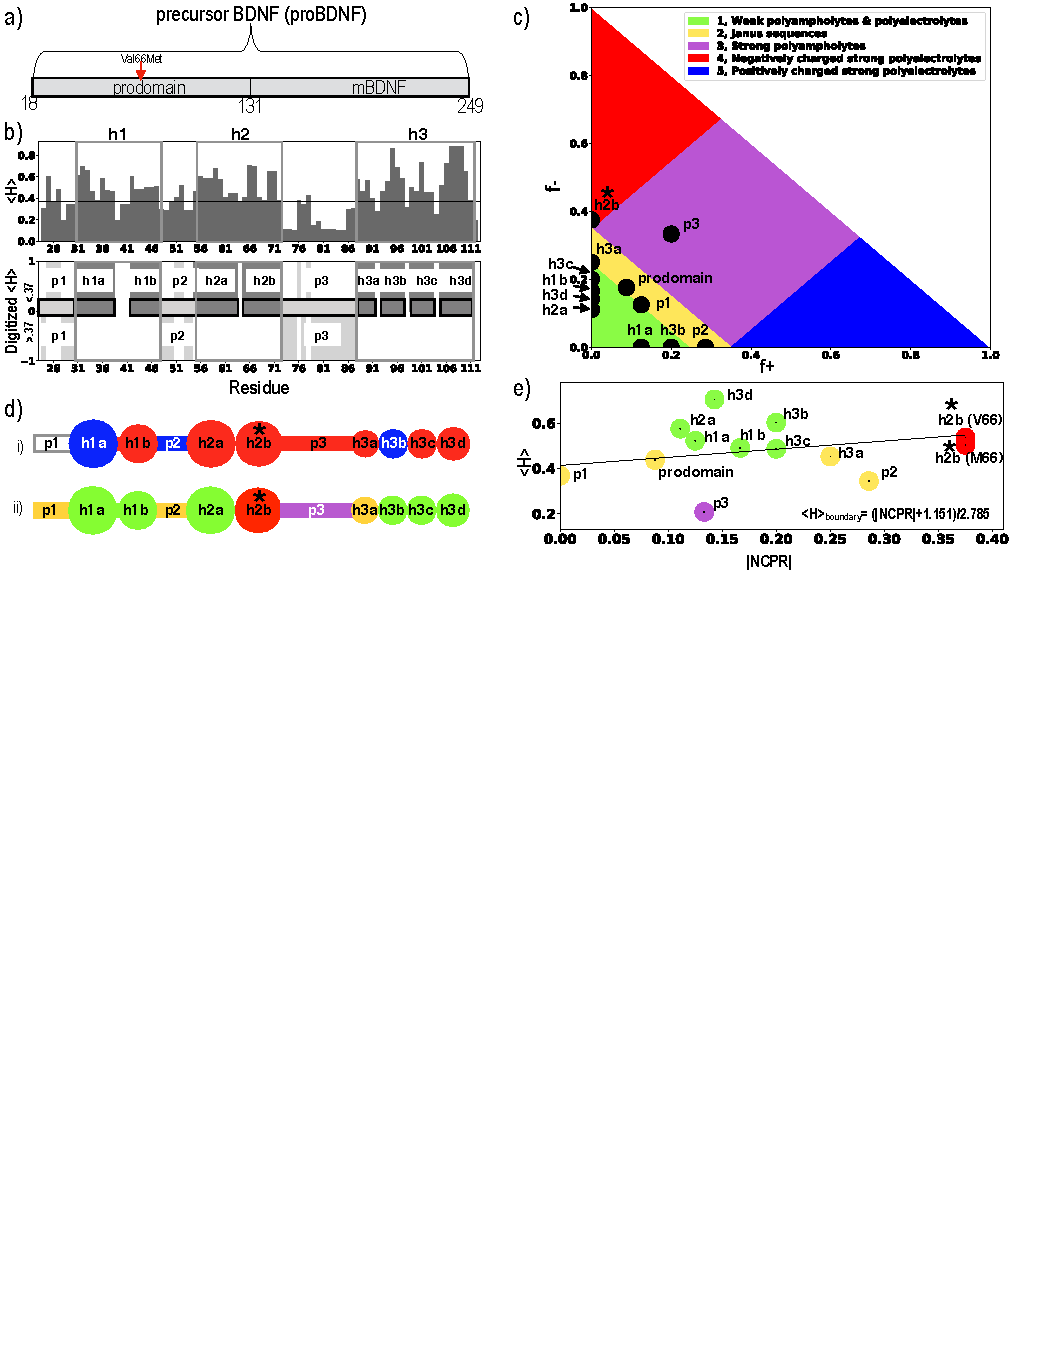
\includegraphics[scale=0.5,width=\textwidth,trim={0 0cm 0 0cm},clip]{../figures/fig1.pdf}
\caption{{\bf Sequence-based decomposition of the BDNF prodomain.} a) The two functional domains of proBDNF: the disordered precursor prodomain considered in this manuscript and the structured mature domain BDNF (mBDNF). b) The mean hydrophobicity $\langle H\rangle$ per residue (top), given by the Kyte-Dolittle\cite{Kyte1982a} score averaged over a three residue window,  and scaled to fit between 0 and 1 was digitized (bottom) according to a cutoff at $\langle H \rangle = 0.37$. Three or more contiguous residues above the cutoff were identified as forming a hydrophobic domain. Eight hydrophobic domains (darkgrey) are identified along with 3 domains of low hydrophobicity (light grey). c) The diagram of IDP states proposed by ~\citeauthor{Das2013a}~\cite {Das2013a}, based on fraction of positive ($f^{+}$) and negative ($f^{-}$) charged residues, and annotated by the location of the whole BDNF prodomain sequence and each subdomain identified in b. d) Domains identified in b), colored according to net charge (i), with negative charge (red), positive charge (blue) and neutral (white) or region of the~\citeauthor{Das2013a} diagram in c) (ii). e) Location of domains on an Uversky diagram~\cite{Uversky2000a} of IDPs and globular proteins, as a function of absolute net charge per residue ($|NCPR|$) and $\langle H\rangle$, with the boundary line between folded and disordered proteins given by the equation in the legend. The domain h2b contains the Val66Met mutation and is marked with star.  Additional properties of the domain sequences can be found in Table 1.}
\label{fig1} 
\end{figure}

Difficulties in obtaining unambiguous disease associations at the proBDNF Val66Met SNP using GWAS are paralleled by challenges in characterizing its effects on the properties of the BDNF prodomain using structural techniques. A crystal structure of a homologous neurotrophic factor in complex with a shared receptor revealed a well-defined volume corresponding to the prodomain, but lacked resolvable density\cite{Feng2010a}.

It was subsequently revealed that the cleaved prodomains ($\sim90$ residues) are found in monomeric states {\it in vivo}, and the M66 (but not V66) form binds to SorCS2 (sortilin-related VPS10p domain containing receptor 2), leading to axonal growth cone retraction\cite{Anastasia2013} and eliminated synapses in hippocampal neurons\cite{Giza2018}. NMR measurements on the prodomain confirmed significant intrinsic disorder for both forms, with differential secondary structure preference around residue 66~\cite {Anastasia2013}.  Tertiary contact distances from NOEs were not accessible, however, and uncertainty in interpretation of the NMR signal obscured non-local effects on secondary structure. Additional NMR experiments implicated residue 66 in binding of M66 prodomain to SorCS2~\cite {Anastasia2013}.
 
%The Val66Met is present in a region with high density of negative charged residues (D61,E64,E68,E69) (Fig~\ref{fig1}c). In this scenario, residue H65 can exist in protonated or neutral charge state in vivo due to it's low pKa. In order to capture the effects of histidine protonation states on Val66Met, we study the Val66 and M66 prodomain in presence of both neutral H65 and protonated H65. For the ease of understanding our observations, the prodomain sequence is divided into hydrophobic domains (Fig~\ref{fig1}c).

In this work, we report on unbiased fully-atomistic replica-exchange MD simulations of the 90 residue BDNF prodomain in explicit solvent, for V66 and M66 forms. This sequence falls in the Janus sequence region in the phase diagram proposed by Das and Pappu\cite{Das2015,Das2013a}. We identify domains using a sequence-based approach based on residue hydrophobicity, which suggests the heterogeneous sequence is composed of multiple globular and intrinsically disordered regions. We then use a hierarchical analysis approach to isolate which interdomain contacts reflect significant effects of the Val66Met substitution, identify the residue level interactions that contribute to these effects, and finally, discuss mechanisms underlying both local and non-local secondary structure effects previously observed through NMR.

\section{Results and discussion}

%%%%%%%%%%%%%%%%%%%%%%%%%%
%1. Definition of Hydrophobic Domains, including some sequence analysis (kappa, f- f+ of individual domains)  (Figure 1)
%2. Comparison of experimental observables and their computational analogues (Figure 2)
%3. Computational Microscopy (expanded data for computational analogues to experimental results)  : Figure 3 and 4
%4. Discussion of Interdomain interactions (prototertiary structure):
%5. Discussion of Intradomain interactions (including length of secondary structures):
%6. Coupling between inter and intradomain interactions

\subsection{Prodomain Sequence Decomposition} 

%This subsection should at minimum answer the following questions : 

%-What was the motivation for dividing into domains (i.e. for coarse-graining the sequence)?
%-How do the different domains correspond to the Pappu phase diagram, and which type of domain does the mutation fall in? 
%-How is the SNP domain unique among the proBDNF domains? How is it that we can have a hydrophobic strong polyelectrolyte sequence? 
%-How are the Pappu domains arranged? (i.e. answer: with strong polyelectrolyte at center and globular domains on ends) 
% -What does coarse-graining the sequence reveal about the proBDNF sequence that isn't apparent from just looking at every residue individually? 

\begin{table}[!ht]
\caption{Sequence based properties of hydrophobic and linker domains identified in the Pro region of BDNF, as shown in Figure \ref{fig1}. }
\label{table1}
\begin{tabular}{|c|c|c|c|c|c|c|c|c|c|c|}
\hline
Domain &  N\textsuperscript{\emph{a}} & NCPR\textsuperscript{\emph{b}}  & $\langle H \rangle$\textsuperscript{\emph{c}}  & FCR\textsuperscript{\emph{d}}  & f-\textsuperscript{\emph{e}} & f+\textsuperscript{\emph{f}} & $\kappa$\textsuperscript{\emph{g}}  & Sequence & R\textsuperscript{\emph{h}} & P\textsuperscript{\emph{i}} \\
\hline\hline
p1 & 8 & 0.00 & 0.37 & 0.25 & 0.13 & 0.13 & 0.8 &  EANIRGQG & 2 & 0.00\\
\hline
h1a & 8 & 0.13 & 0.52 & 0.13 & 0.00 & 0.13 & 1.0 &  GLAYPGVR & 1 & 0.13\\
\hline
h1b & 6 & -0.17 & 0.49 & 0.17 & 0.17 & 0.00 & 0.1 &  TLESVN & 1 & 0.00\\
\hline
p2 & 7 & 0.29 & 0.34 & 0.29 & 0.00 & 0.29 & 1.0 &  GPKAGSR & 2 & 0.14\\
\hline
h2a & 9 & -0.11 & 0.58 & 0.11 & 0.11 & 0.00 & 0.7 & GLTSLADTF & 1 & 0.00\\
\hline
h2b(V66) & 8 & -0.38 & 0.54 & 0.38 & 0.38 & 0.00 & 0.3 &  HVIEELLD & 4 & 0.00\\
\hline
h2b(M66) & 8 & -0.38 & 0.50 & 0.38 & 0.38 & 0.00 & 0.3 &  HMIEELLD & 4 & 0.00\\
\hline
p3 & 15 & -0.13 & 0.21 & 0.53 & 0.33 & 0.20 & 0.1 & \makecell{EDQKVRP \\ NEENNKDA} & 3 & 0.06\\
\hline
h3a & 4 & -0.25 & 0.45 & 0.25 & 0.25 & 0.00 & N/A &  DLYT & 2 & 0.00\\
\hline
h3b & 5 & 0.20 & 0.60 & 0.20 & 0.00 & 0.20 & N/A &  RVMLS & 1 & 0.00\\
\hline
h3c & 5 & -0.20 & 0.49 & 0.20 & 0.20 & 0.00 &N/A &  QVPLE & 1 & 0.20\\
\hline
h3d & 7 & -0.14 & 0.70 & 0.14 & 0.14 & 0.00 & 1.0 &  PLLFLLE & 1& 0.14\\
\hline\hline
V66 Seq  & 91 & -0.09 & 0.44 & 0.26 & 0.18 & 0.09 & 0.2 & & 2 &0.07 \\
\hline
M66 Seq & 91 & -0.09 & 0.43 & 0.26 & 0.18 & 0.09 & 0.2 & & 2 &0.07 \\
\hline
\end{tabular}
\begin{flushleft}
\textsuperscript{\emph{a}} Number of residues in the domain\\
\textsuperscript{\emph{b}} Net charge per residue\\
\textsuperscript{\emph{c}} Mean hydrophobicity, average of Kyte-Dolittle \cite{Kyte1982a} scores for each residue in the domain scaled to fit between 0 and 1  \\
\textsuperscript{\emph{d}} Fraction of charged residues\\
\textsuperscript{\emph{e}} Fraction of positively charged residues\\
\textsuperscript{\emph{f}}  Fraction of negatively charged residues\\ 
\textsuperscript{\emph{g}} Charge distribution parameter $\kappa$ as defined by Das and Pappu \cite{Das2013a}, calculated using CIDER~\cite{Holehouse2017} \\
\textsuperscript{\emph{h}} Region in phase diagram proposed by Das and Pappu \cite {Das2013a}, (Figure~\ref{fig1}c)\\
\textsuperscript{\emph{i}} Fraction of Proline residues\\
\end{flushleft}
\end{table}

The region of the BDNF prodomain studied using NMR\cite{Anastasia2013}, and simulated here, is 91 residues long. The potential number of residue-residue contacts is $91\times90/2\sim4000$, and each contact is formed infrequently. Detecting significant differences for numerous weak signals is statistically prohibitive, even given the long simulations presented here. We were initially motivated to divide the sequence into domains based on sequence hydrophobicity, as described in Methods, to address this analysis challenge (Figure~\ref{fig1}b). Such coarse-graining reduces the number of potential contacts to $11\times10/2=55$, while increasing the likelihood that any given contact will be formed. Three hydrophobic macrodomains were identified (Figure~\ref{fig1}b): h1, h2, and h3. The h domains are separated by three charged linker  (``p'') domains : p1, p2, and p3.  Each h macrodomain contains two to four microdomains, separated by one or two residues each:  h1 contains h1a and h1b,  h2 contains h2a and h2b, and h3 contains h3a, h3b, h3c, and h3d.  

Since each domain sequence has its own properties (Table ~\ref{table1}), this process also suggested a new, more tractable conceptualization of the long, disordered BDNF prodomain. Each domain can be analyzed individually according to \citeauthor{Das2013a} metrics~\cite{Das2013a} (Figure~\ref{fig1}c) or Uversky metrics~\cite {Uversky2000a} (Figure~\ref{fig1}e), while several other sequence properties of each domain are shown in Table~\ref{table1}. %  charge distribution parameter $\kappa$ ~\cite {Das2013a} and fraction of Proline residues (P) . 
The \citeauthor{Das2013a} phase diagram~\cite{Das2013a} predicts the compactness of IDPs based on their fraction of positively (f+) and negatively (f-) charged residues (Figure~\ref{fig1}c). Hydrophobic domains h2b and domain h3a lie in the strong polyelectrolyte and Janus sequence region respectively. All the remaining hydrophobic domains are classified as weak polyampholyte and, as isolated peptides, would be predicted to have compact globule conformations to shield hydrophobic residues~\cite{Das2013a}. Linkers p1 and p2 also lie in the Janus sequence regions, while linker p3 lies in the strong polyampholyte region with low value of the charge distribution parameter $\kappa$~\cite{Das2013a}, and is predicted to have random coil conformations if present as an isolated peptide.

The Uversky diagram~\cite{Uversky2000a} characterizes proteins as globular or intrinsically disordered based on their normalized mean hydrophobicity and absolute net charge per residue ($|NCPR|$) (Figure~\ref{fig1}e). The proteins falling above the boundary line are classified as globular proteins, while the ones below that line are generally classified as IDPs. With the exception of hydrophobic domains h2b and h3a, all hydrophobic domains identified here fall in the globular protein regions. Domains h2b, h3a and p1 fall on the disordered side of the boundary, while p2 and p3 are both deep in the disordered region.

%Two unique domains with high NCPR ($\geq$ 0.25) and hydrophobicity ($\geq$ 0.45) are identified; h2b and h3a. 

The domain h2b containing Val66Met has several unique properties among the identified domains: 1) it is located at the sequence midpoint 2) it is the only strong polyelectrolyte domain 3) it has the strongest NCPR (-0.38) among all the domains 4) The sequence is composed almost entirely of two competing residue types, yielding the uncommon mix of a highly-charged, hydrophobic domain. Considering mean hydrophobicity alone, \citeauthor{Uversky2000a}\cite{Uversky2000a}  found $\langle H \rangle\sim 0.48 \pm{� 0.03}$ for a set of 275 folded proteins and $\langle H \rangle\sim  0.39 \pm{� 0.05}$ for a set of 91 unfolded proteins. By this criteria, we would expect the h2b sequence to be folded: for V66-h2b, $\langle H \rangle \sim 0.54$, while for M66-h2b,  $\langle H \rangle\sim0.50$. The full Uversky diagram also considers NCPR, and the strong NCPR pushes h2b into the IDP region of the Uversky diagram~\cite{Uversky2000a}. 

More specifically, this domain sequence (HV/MIEELLD) has hydrophobic residues at i, i+3, i+4 separated by acidic residues at i+1, i+2.  Helix formation would thus segregate hydrophobic residues from acidic residues but would also increase the density of like-charge residues. Similar sequences are observed in the activation domains of transcription factors: a motif of alternating hydrophobic and acidic residues folds into an amphipathic helix upon binding, and the interactions between the amphipathic helix and the binding partner are mediated by hydrophobic residues, not charged residues~\cite{Brzovic2011,Uesugi1997, Radhakrishnan1997, Canales2017, Staller2018}.  ~\citeauthor{Staller2018}~\cite {Staller2018} have earlier reported that in the disordered acidic activation domain of Gcn4, the acidic residues keep key hydrophobic residues exposed to solvent and binding partners.
% It has been repeatedly observed that several IDPs mediate their interactions with their binding partners with hydrophobic residues ~\cite{Santofimia-Castano2017,Uesugi1997, Radhakrishnan1997, Canales2017, Staller2018}. 
%Santofimia-Castano et al ~\cite{Santofimia-Castano2017} showed that NUPR1 sequence interacts with several biomolecules through hydrophobic patches on it's surface. 

The domain h3a is a unique hydrophobic Janus domain with high NCPR. Janus sequences have intermediate compositional biases and their conformations are  context dependent\cite{Das2013a, Das2015b}. The SNP domain h2b and the Janus domain h3a are separated by the long (15 residue) strong polyampholyte linker p3, which has well mixed charge ($\kappa$ = 0.1). The domains h1a and h3b are positively charged and all the remaining hydrophobic domains are negatively charged (Figure~\ref{fig1}d).

%Forty percent of IDPs reported in DISPROT are found to have compositions that place them in the boundary between globules and strong polyampholytes ~\cite {Das2015b}. 

%%%%%%%%%%%%%%%%%%%%%%%%%%%%%%
\subsection{Comparison of experimental observables and their computational analogues}

NMR chemical shifts (Figure~\ref{fig2}a) for the Val66 and M66 prodomain indicated that they are disordered, lacking any stable secondary structure~\cite{Anastasia2013}. Many of the common force-field and water model combinations used for MD simulations are optimized for folded proteins, and are not recommended for IDPs~\cite{Mercadante2015,Piana2015}. Piana el al~\cite{Piana2015} showed that several such force-field and water model combinations produced substantially more compact disordered states when compared with experiments. In order to predict accurate ensembles of the prodomain, we tested several force-field and water model combinations, optimized for IDPs, including Amberff03sbws~\cite{Best2009, Best2014} with TIP4P/2005~\cite{Abascal2005}, Amber99sbws~\cite{Lindorff-Larsen2010a, Best2014} with TIP4P/2005~\cite{Abascal2005} and Amber99sb*-ildn-q~\cite{Lindorff-Larsen2010a, Hornak2006a} with Tip4p-D~\cite{Piana2015}, on 30 residue fragments of the V66 prodomain using temperature replica exchange molecular dynamics (T-REMD), further described in SI. Amber99sb*-ildn-q~\cite{Lindorff-Larsen2010a, Hornak2006a} with Tip4p-D~\cite{Piana2015} yielded the best agreement with experimental data obtained by NMR~\cite{Anastasia2013} (FigureS1) and was used for the full prodomain MD simulations further described in Methods. This is consistent with the force field comparison study by ~\citeauthor{Robustelli2018}, which observed that for IDPs with little or no secondary structure, Amber99sb*-ildn-q with Tip4p-D gives best agreement with experimental NMR measurements~\cite{Robustelli2018}.
\begin{figure}[!ht]
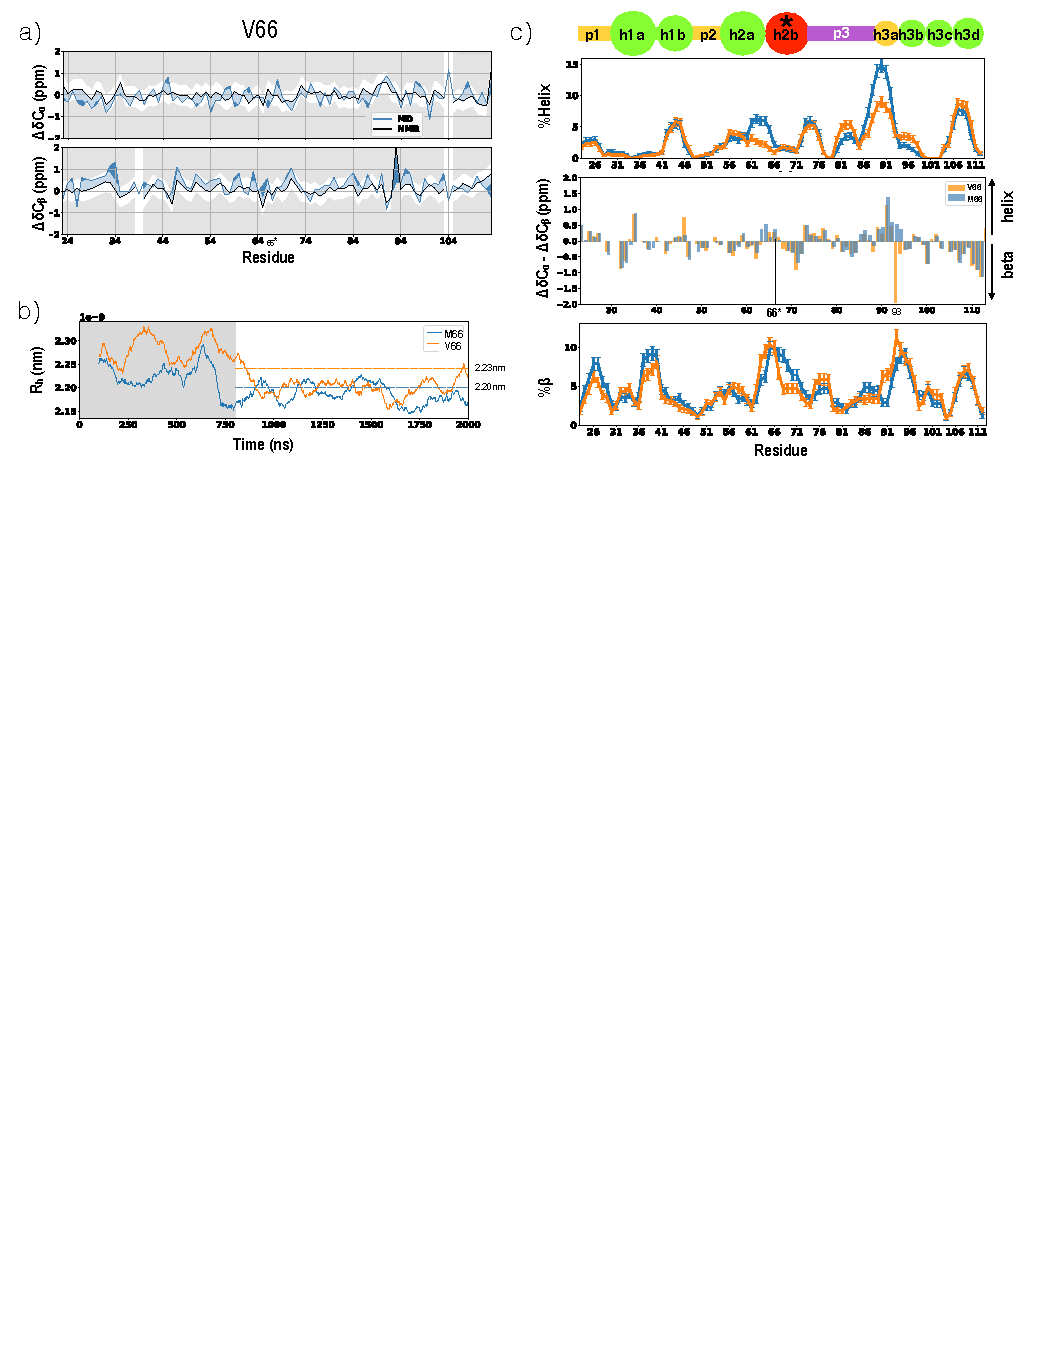
\includegraphics[scale=0.5,width=\textwidth,trim={0 0cm 0 0cm},clip]{../figures/fig2.pdf}
\caption{{\bf Comparison of MD and NMR observables.} a) Chemical shifts from NMR at 280K (black lines)~\cite{Anastasia2013} and MD at 300K (blue lines), calculated using SPARTA+ ~\cite{Shen2010}. The gray region represents a discrepancy of more than 0.5 ppm from NMR chemical shifts. b) Hydrodynamic radius ($R_{h}$) vs the simulation time, using a 100 ns moving window. The NMR diffusion experiment values~\cite{Anastasia2013} are represented with dashed lines, and the shaded region represents the discarded equilibration period. c) Helix (top) or $\beta$ (bottom) propensity at each simulated residue, defined as the probability of a given residue being part of a sequence of four or more consecutive residues whose dihedral angles place them in the helical (top) region or beta (bottom) region of the Ramachandran map (further described in methods). C\textsubscript{$\alpha$}-C\textsubscript{$\beta$} secondary chemical shifts for each sequence from ~\citeauthor{Anastasia2013}~\cite{Anastasia2013} (middle) are also shown. Positive differences indicate helical structure and negative differences indicate $\beta$ structure. Errors represent standard error of a Bernoulli trial with n number of samples, where n is the product of total number replicas, 64 and average number of roundtrips per replica, 17.}
\label{fig2} 
\end{figure}


In order to assess the validity of MD-generated ensembles, we compared the MD ensembles with experimental data obtained by NMR spectroscopy and NMR diffusion measurements. Figure~\ref{fig2}a shows the C\textsubscript{$\alpha$} and C\textsubscript{$\beta$} chemical shifts calculated from the simulations using SPARTA+~\cite{Shen2010} and compares them with the NMR chemical shifts obtained from~\citeauthor{Anastasia2013}~\cite{Anastasia2013} for V66 sequence and M66 sequence (Figure S2). We obtain good agreement with NMR chemical shifts: the discrepancy at each residue is \textless 0.7 ppm, which is less than the individual SPARTA+ prediction uncertainties of $\sim$ 1 ppm~\cite{Shen2010}. 
%Although for C\textsubscript{$\beta$} chemical shifts there are some localized discrepancies for certain residue types (Y34,L59,M95,Y113), the discrepancy is conserved across both the simulations (FigureS2). Thus, these specific discrepancies are probably reflecting residual force-field inaccuracies, including the cation-pi interactions that are poorly captured by non-polarizable force field.

The simulated hydrodynamic radii ($R_{h}$) calculated using Hydropro~\cite{Ortega2011} for both the V66 ($R_{h}=2.23 \pm 
  { .01}$ nm) and M66 ($R_{h}=2.20 \pm  {  .01}$ nm) sequences are in excellent agreement with the experimental values from NMR diffusion measurements~\cite{Anastasia2013} ($R_{h}=2.24 \pm { 0.1}$ nm and $R_{h}=2.20\pm {0.1}$ nm for the V66 and M66 sequence respectively) (Figure~\ref{fig2}b). Comparison between $R_h$ generated from MD and NMR/SAXS experiments has been used earlier to validate simulations of disordered proteins~\cite{Mercadante2015, Rauscher2015, Meng2018} and our results support the use of Tip4p-D for such simulations~\cite{Piana2015, Robustelli2018}. Use of Tip3P resulted in more compact ensembles (data not shown). The simulated radius of gyration ($R_g$) distribution for both the V66 and M66 sequences demonstrate that both prodomains populate closely overlapping ensembles (Figure~\ref{fig3}a).  

~\citeauthor{Anastasia2013}~\cite{Anastasia2013} observed an increase in helical tendency for the M66 sequence within domain h2 and h3ab and an increase in $\beta$ tendency within domain h3b in the V66 sequence (Figure~\ref{fig2}c). Consistent with NMR experiments~\cite{Anastasia2013}, the M66 sequence demonstrates an increased tendency of forming helices within domain h2 and h3a relative to the same domains in the V66 sequence (Figure~\ref{fig2}c). We also find that the residue R93 in domain h3b of V66 sequence has a  $\sim$ 30\% higher tendency to form $\beta$-sheets than in the M66 sequence, in agreement with NMR experiments.
 
%%%%%%%%%%%%%%%%%%%%
\subsection{Heterogeneous behavior of individual domains}

Disordered proteins can be well-described by Flory scaling theory $\langle R_{|i-j|}\rangle =  An^{\nu}$, where $\langle R_{|i-j|}\rangle$ is the ensemble-averaged internal distance, $|$i-j$|$ is residue separation along the chain, and $\nu$ is the Flory scaling coefficient\cite{Flory1949}. Larger values of $\nu$ correspond to swollen coils, while smaller values correspond to compact globules\cite{Das2013a}. In particular, when $\nu$=0.6 (``good solvent") the protein maximizes its interaction with solvent, and for  $\nu$=0.33 (``poor solvent"), the protein maximizes self-interactions. The special intermediate case of $\nu$=0.5 is called a ``theta solvent"\cite{Flory1949}. Most IDPs that obey this scaling behavior have $\nu$$>$0.5\cite{Hofmann2012,Das2013a,Zerze2015,Meng2018}. As shown in Figure~\ref{fig3}b, the prodomain as a whole is not well fit by a single power law: for separations of 15 or fewer residues the prodomain falls in the ``theta solvent" regime, while for separations of 20 or more residues it falls in the ``poor solvent" regime.

\begin{figure}[!ht]
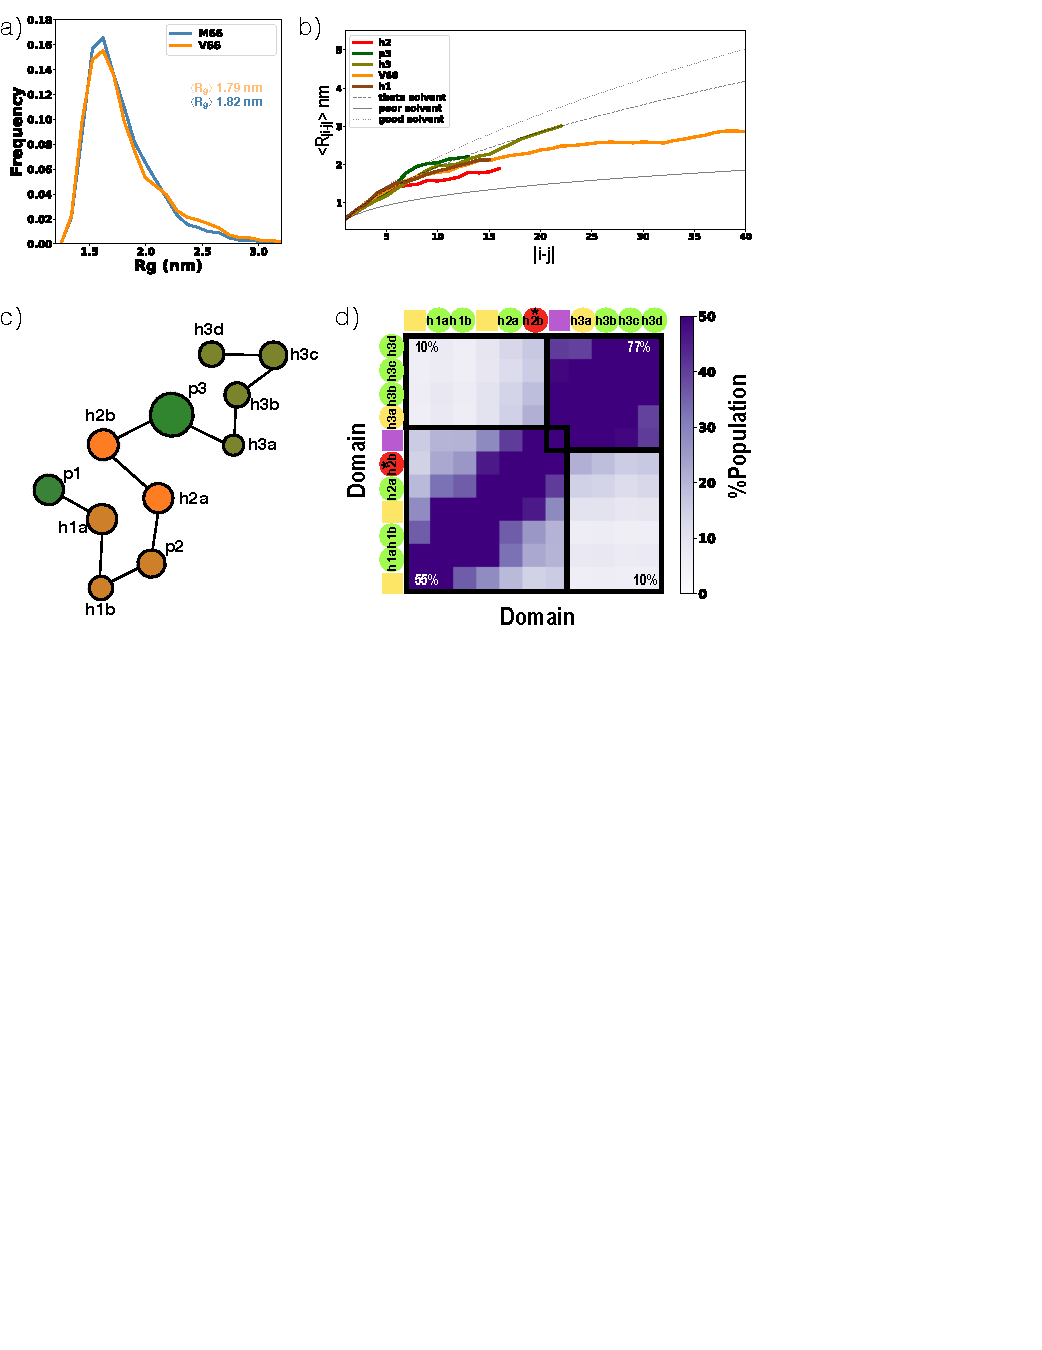
\includegraphics[scale=0.5,width=0.9\textwidth,trim={0 0cm 0 0cm},clip]{../figures/fig3.pdf}
\caption{{\bf Heterogeneity in the BDNF prodomain.} a) $R_g$ distributions for the V66 and M66 sequence, with $\langle R_{g,M66}\rangle= 1.79 \pm {0.01}$ nm and $\langle R_{g,V66}\rangle = 1.82 \pm {0.01}$ nm. b) Ensemble averaged intrachain distance profiles for the V66 sequence,  as well as each hydrophobic macro-domain and the disordered p3 linker. Theoretical polymer scaling limits are shown with dashed lines (prefactor A = 0.55 nm) while Flory exponents for each curve are given in Table \ref{table2}.  c)   Model for the freely-jointed self-avoiding heteropolymer mimicking the BDNF prodomain, drawn to scale, with the size and separation between beads reflects $R_g$ and $R_{\mathrm{etoe}}$ for each domain (Table~\ref{table2}). The domains are colored according to their Flory exponents:  $\nu$$>=$0.6 is green, $\nu$$<=$0.45 is orange and the remaining  $\nu$ in the ``theta solvent" range is colored brown.  d) Inter-domain contact probability for the model in (c), calculated as described in Methods. The black boxes mark the regions on either side of the h2b-p3 boundary, and each is annotated with the average contact probability for any domain-pair falling within it.} 
\label{fig3}
\end{figure}


\begin{table}[!ht]
\caption{Average radius of gyration ($R_g$), Average end to end distance ($R_{\mathrm{etoe}}$) and Flory exponent ($\nu$) for each proregion domain, calculated from MD trajectories. Errors represent fit error of $\langle R_{|i-j|}\rangle$ vs  $An^{\nu}$, weighted by each point's standard deviation. Values for V66 and M66 sequences were within error.}
\label{table2}
\begin{tabular}{|c|c|c|c|c|}  
\hline 
Domain & $\langle R_g \rangle $ (nm)  & $\langle R_{\mathrm{etoe}} \rangle$ (nm)  & $\nu$ (V66) & $\nu$ (M66)  \\
\hline
p1 & 0.67 $\pm{0.01}$ & 1.60 $\pm{0.05}$ & &\\
\hline
h1a & 0.67 $\pm{0.01}$ & 1.60 $\pm{0.06}$ &  \multirow{2}{*}{0.49  $\pm{0.11}$} &  \multirow{2}{*}{0.53  $\pm{0.11}$} \\ \cline{1-3}
h1b & 0.53 $\pm{0.01}$ & 1.21 $\pm{0.04}$  & &\\
\hline
p2 & 0.62 $\pm{0.01}$ & 1.38 $\pm{0.05}$ & &\\
\hline
h2a & 0.66 $\pm{0.01}$ & 1.47 $\pm{0.06}$ & \multirow{2}{*}{0.42 $\pm{0.11}$} & \multirow{2}{*}{0.43  $\pm{0.11}$}\\  \cline{1-3}

h2b & 0.68 $\pm{0.01}$ & 1.80 $\pm{0.05}$ & &\\ 
\hline
p3 & 0.97 $\pm{0.01}$ & 2.16 $\pm{0.08}$  & 0.63  $\pm{0.10}$ &  0.62   $\pm{0.10}$\\
\hline
h3a & 0.46 $\pm{0.00}$ & 0.93 $\pm{0.02}$ & \multirow{4}{*}{0.58 $\pm{0.08}$} & \multirow{4}{*}{0.54   $\pm{0.08}$}\\ \cline{1-3}

h3b & 0.55 $\pm{0.01}$ & 1.23 $\pm{0.03}$ & &\\ 

h3c & 0.56 $\pm{0.00}$ & 1.27 $\pm{0.03}$ & & \\ 

h3d & 0.62 $\pm{0.01}$ & 1.53 $\pm{0.04}$ & &\\
\hline
\end{tabular}
\end{table}

Each identified individual domain does obey a power law, and we calculated A and $\nu$ for each domain as if it was isolated from rest of the protein (Table S1, Figure S3). For every domain except the p3 linker, the error across $\nu$ values was substantial, since N was short. However, each hydrophobic macro-domain h1,h2 and h3 can be fit by a power law, with the Flory exponents shown in Table~\ref{table2}. The lowest observed value of $\nu$ was observed in h2  ($\nu = 0.42 \pm 0.11$) and the highest value was in the adjacent p3 domain ($\nu = 0.63 \pm 0.1$), suggesting a sharp boundary at the h2-p3 interface, where the sequence shifts from highly collapsed (``poor solvent") to highly expanded (``good solvent") tendencies.

% For domain h2 the value of $\nu$ ($\nu$=0.42 $\pm { 0.1}$), is most compact among all three hydrophobic domains, and lies between poor and theta solvent. For p3, $\nu$= 0.63 $\pm { 0.1}$, reaches the good solvent limit, which is consistent with the low hydrophobicity and expanded (excluded volume limit) coil conformations as predicted from phase behavior of a strong polyampholyte with low $\kappa$~\cite {Das2013a} (Table~\ref{table2}). 

We expect that even for a heterogeneous freely-jointed, self-avoiding polymer, contact probability between monomers would depend on monomer shape and separation. To predict the inter-domain contact probability for a self-avoiding polymer composed of 11 monomers with properties similar to our domains (analogous to Kuhn segments\cite{Rubinstein2003}), we performed simple Monte Carlo calculations as described in methods. The monomer-monomer bond length (analogous to the Kuhn length) and excluded volume radius reflected the average end to end distance ($R_{\mathrm{etoe}}$) and radius of gyration ($R_{g}$) for each domain from MD simulations (Table~\ref{table2}), and a schematic drawn to scale is shown in Figure \ref{fig3}c. The predicted interdomain contact probabilities for this freely-jointed, self-avoiding heteropolymer are shown in Figure~\ref{fig3}d, suggesting that such a chain would effectively be segmented at the boundary between the domains mimicking h2b and p3.  More specifically, domains on the N terminal side of p3 are in contact in 55\% of the frames, while domains on the C terminal side are in contact in 77\% of the frames, but the average contact probability between these two self-interacting regions is 10\%.  Shifting the p3 bead within the chain shifts the boundary (Figure S4). These calculations provide a useful reference expectation for interpreting interdomain contacts in the real sequence.

\subsection{Interdomain and tertiary interactions}

%--------- domain level
%change the cutoff in contact maps
%--Purely based on the domain properties (not individual residue stuff yet), what interdomain interaction preferences would we expect (if any)?
%--What do we actually observe (in the WT, ancestral version)
%--Does it agree with our expectation?
%--How does the V66M hydrophobic mutation change these preferential interactions?  (Not "why" yet, just how)
%--V66M doesn't change any of the domain properties (does it?) - is there still a way for us to interpret  preferential interactions purely on the domain level? (i.e. h3a  is Janus sequence which is highly sensitive to small changes in interactions)
%--How does  65+  change  interdomain interactions, and is it consistent with what we'd expect based on how it affects properties of domain 2b?
%--Are changes in interdomain interactions consistent with changes in radius of gyration?
%a metric for the strongest contact formed in each domain

\begin{figure}[!ht]
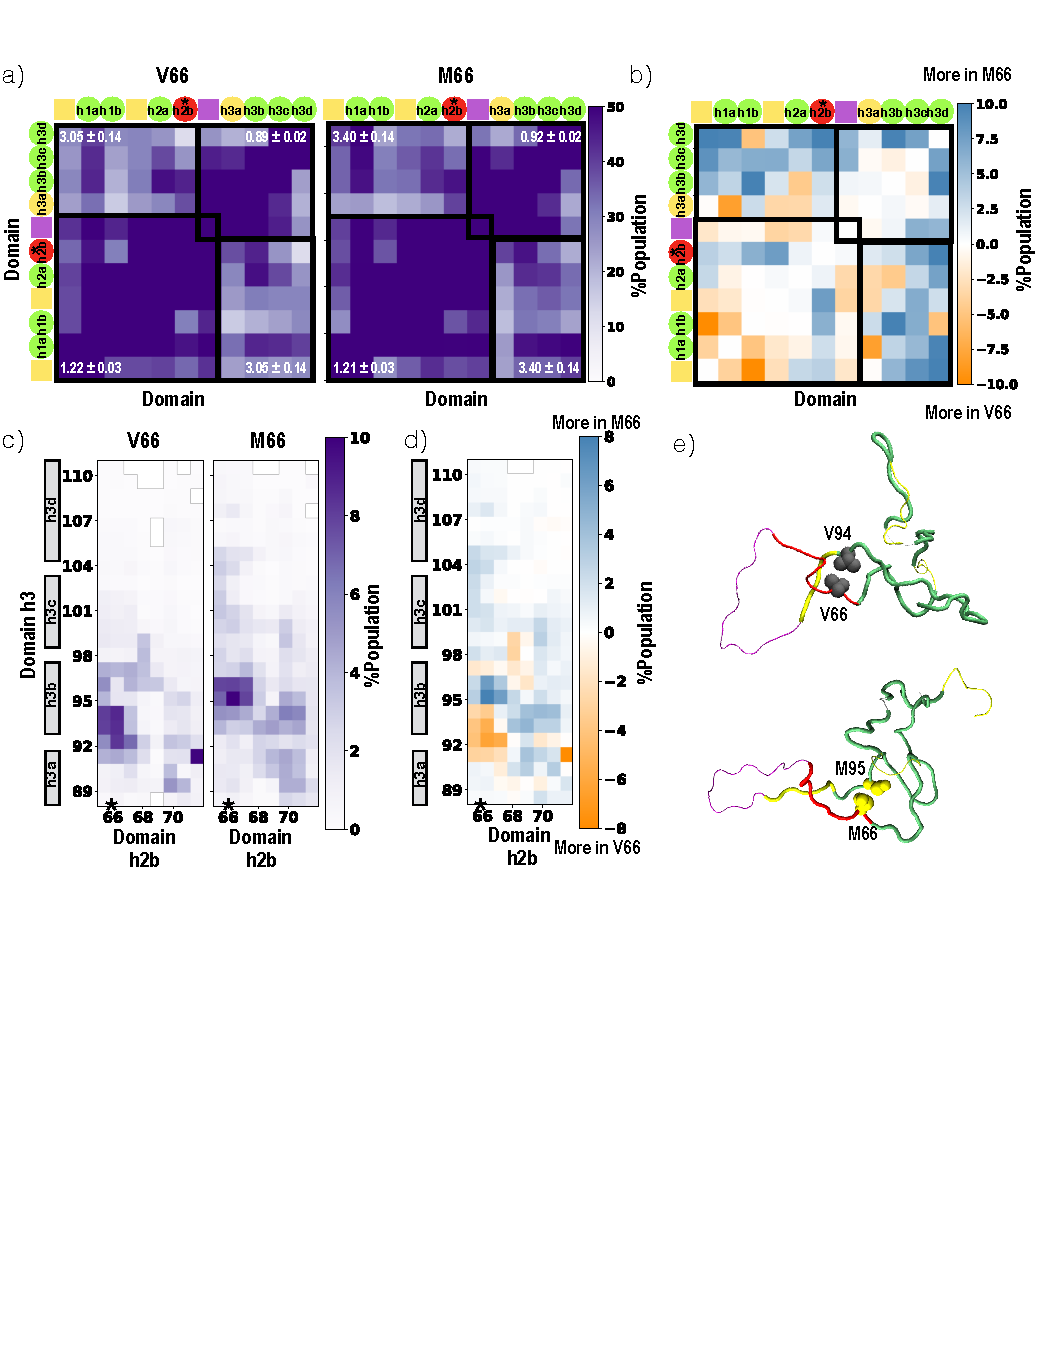
\includegraphics[scale=0.3,width=\textwidth,trim={0 0cm 0 0cm},clip]{../figures/fig4.pdf}
\caption{{\bf Effect of Val66Met on inter-domain contacts.} a) Inter-domain contact probability for the V66 (left) and M66 (right) sequences, calculated as described in Methods. The black boxes mark the regions identified in Figure \ref{fig3}d for the self-avoiding heteropolymer, and the enrichment for the total number of contacts, relative to the totals in Figure \ref{fig3}d, are annotated for each box. The errors represent standard errors (n =1088 as described in Methods). The x and y axes are annotated with cartoon representations of the prodomain; circles and squares represent hydrophobic domains and linker regions respectively and are colored as in Figure 1. %Two domains are in contact if the excess distance between them is at least 0.55nm, as described in Methods.
b) Difference between the contact probabilities shown in a); interactions more frequently found in M66 or V66 are in blue and orange respectively. c) Contact probability at each residue in h2b with each residue in h3 for V66 (left) and M66 (right). d) Difference between the contact probabilities shown in c); interactions colored as in b). e) Representative conformation of V66 sequence (top) and M66 sequence (bottom) showing Val66-Val94 and Met66-Met95 contact respectively, colored as in Figure1 with Methionine in yellow. Tubes represent hydrophobic domains whereas lines represents linker regions.}
 
\label{fig4}
\end{figure}

Figure \ref{fig4}a shows the probability of interdomain contacts for both the V66 and M66 sequences, calculated analogously to those in the self-avoiding heteropolymer in Figure \ref{fig3}d. Consistent with the MC predictions, the contact probability map for each sequence clusters into 4 visible regions, separated along both axes by domain p3. The total number of interdomain contacts that did not cross the boundary were quantitatively consistent with the self-avoiding heteropolymer, exhibiting frequencies that were only 20\% more and 10\% less than the self-avoiding heteropolymer frequencies on the N-terminal and C-terminal side respectively. These frequencies were the same for both the V66 and M66 sequences.    

In the real protein, contacts crossing the h2-p3 boundary are much less common than those on either side of the boundary, which is qualitatively consistent with the predictions for the self-avoiding heteropolymer (Figure \ref{fig4}a). Quantitatively, they are still about three times more common than predicted from the self-avoiding heteropolymer, consistent with favorable interdomain interactions across the boundary.  Furthermore, the extent of enrichment changes with the Val66Met mutation: the V66 sequence has 3.1$\times$ enrichment while the M66 sequence has 3.4$\times$ enrichment. The increased number of cross-boundary contacts are also consistent with the lower mean hydrodynamic radius (Figure~\ref{fig2}b) and radius of gyration (Figure~\ref{fig3}a) for the M66 sequence. 

This difference suggested that the presence of residue 66 near the collapsed/expanded boundary could contribute to its conformational effects, and consistent with this hypothesis, the M66-h2b domain contacts every domain on the other side of the boundary more frequently than does the V66-h2b domain (Figure~\ref{fig4}b). 
%As shown in Figure 3a, the most frequent contacts we observed between non-neighboring domains were h1a-h3abc and h2b-h3ab. Seven out of 11 domains in the prodomain are negatively charged and only 2 domains(h1a and h3b) are positively charged (Table~\ref{table1}), so the high frequency of contacts involving either h1a or h3b is consistent with a role for electrostatic contributions, even between hydrophobic domains. 

To understand the origin of the favorable interaction between the SNP domain h2b and the C-terminal side of p3, we consider the contacts between the residues of these domains (Figure~\ref{fig4}c, Figure S5). As shown in the absolute contact probability map (Figure~\ref{fig4}c), the SNP domain h2b forms most frequent contacts with domain h3b in the C-terminal side of p3. At residue level, both sequences frequently form contacts between hydrophobic residues at domains h2b-h3b, but the residue pairs most frequently forming the contact shift from Val66-Val94 in the V66 sequence to Met66-Met95 in the M66 sequence (Figure~\ref{fig4}c and d). This result was remarkably consistent with a role for residue 66 in driving these interdomain interactions, as well as sensitivity to the Val66Met substitution.  

Specific Met-Met interactions between the two polarizable sulfur atoms are often under appreciated, but are common in structures of folded proteins\cite{Faure2008}. Using ab initio calculations, \citeauthor{Gomez-Tamayo2016} predicted that Met-Met interactions are stronger than Met-aromatic or aromatic-aromatic interactions~\cite{Gomez-Tamayo2016}. These interactions are also captured reasonably well in the non-polarizable AMBER force field~\cite{Gomez-Tamayo2016}. In these simulations, the Met66-Met95 contact was about five times as common (10\% of frames) as the analogous Val66-Met95 contact (2\% of frames).  Methionine-aromatic interactions also contribute to the increased number of cross boundary contacts:  M66, but not V66, forms a frequent contact with F108 in domain h3d, which is also consistent with the favorable interactions between Met-Phe residues\cite{Viguera1995,Faure2008,Valley2012} (Figure \ref{fig4}d). While determining intermolecular interactions that cause compaction in the disordered domain of poly(A)-binding protein using small-angle X-ray scattering (SAXS), Riback2017 et al.~\cite{Riback2017} reported that increasing the net hydrophobicity produces increased domain compaction across multiple sets of mutations, with one exception: substituting the less hydrophobic Methionine with more hydrophobic Valine. 

%We calculated the differences in contact probability at each residue between these two domains(Figure~\ref{fig4}d). We find that mutations residue M66 within domain h2b specifically forms strongest contacts with domain h3b and h3d. Interestingly, we find that Met95 forms frequent contacts with Met66 and not Val66 (Met66-Met95 (10\%) vs Val66-Met95 (2\%)). This is consistent with the results of ab-initio calculations: Gomez-Tamayo et al has reported that Met-Met interactions are stronger than Met-Leu, Met-Phe or aromatic-aromatic interactions due to polarizability of sulphur ~\cite{Gomez-Tamayo2016}. These interactions are also captured reasonably well in the AMBER force field ~\cite{Gomez-Tamayo2016}. In domain h3d, F108 forms strong contact with M66 and not V66, which is also consistent with the favorable interactions between these Met-Phe residues \cite{Viguera1995,Faure2008,Valley2012}. 

%For the M66 sequence, the SNP domain h2b gains contacts with all other domains relative to V66 (Figure~\ref{fig4}b). This is consistent with the lower average $R_h$ (Figure~\ref{fig2}b) and $R_g$ (Figure~\ref{fig3}a) observed for the M66 sequence in both experiments and simulations. 
%note earlier rebeca et al also observed that M is more collapsed than V but the reason was not understood.

%%%%%%%%%%%%%%%%%%%%%%%%%%%%%%%%%%%%INTRADOMAIN%%%%%%%%%%%%%%%%%%%%%%%%%%%%%%
\subsection{Intradomain interactions and residual secondary structure}

NMR chemical shifts~\cite{Anastasia2013} indicate that the Val66Met mutation increases the helicity within both the SNP domain h2b and Janus domain h3a. In agreement with NMR, we find an increase in helical structure at both domains in the M66 sequence (Figure~\ref{fig2}c). Comparing the length of secondary structure formed at each residue (Figure~\ref{fig5}a and c) reveals an even stronger effect of the mutation that would not have been detectable via NMR: Val66Met consistently increases the frequency of long helices formed within domain h2. 
%Strikingly, we find that only Met66 and not V66 forms long helical structures of 4 or more residues at the SNP domain (2a,2b) (Figure~\ref{fig4}a). We observe likewise for M\textsuperscript{65+}. 

\begin{figure}[!ht]
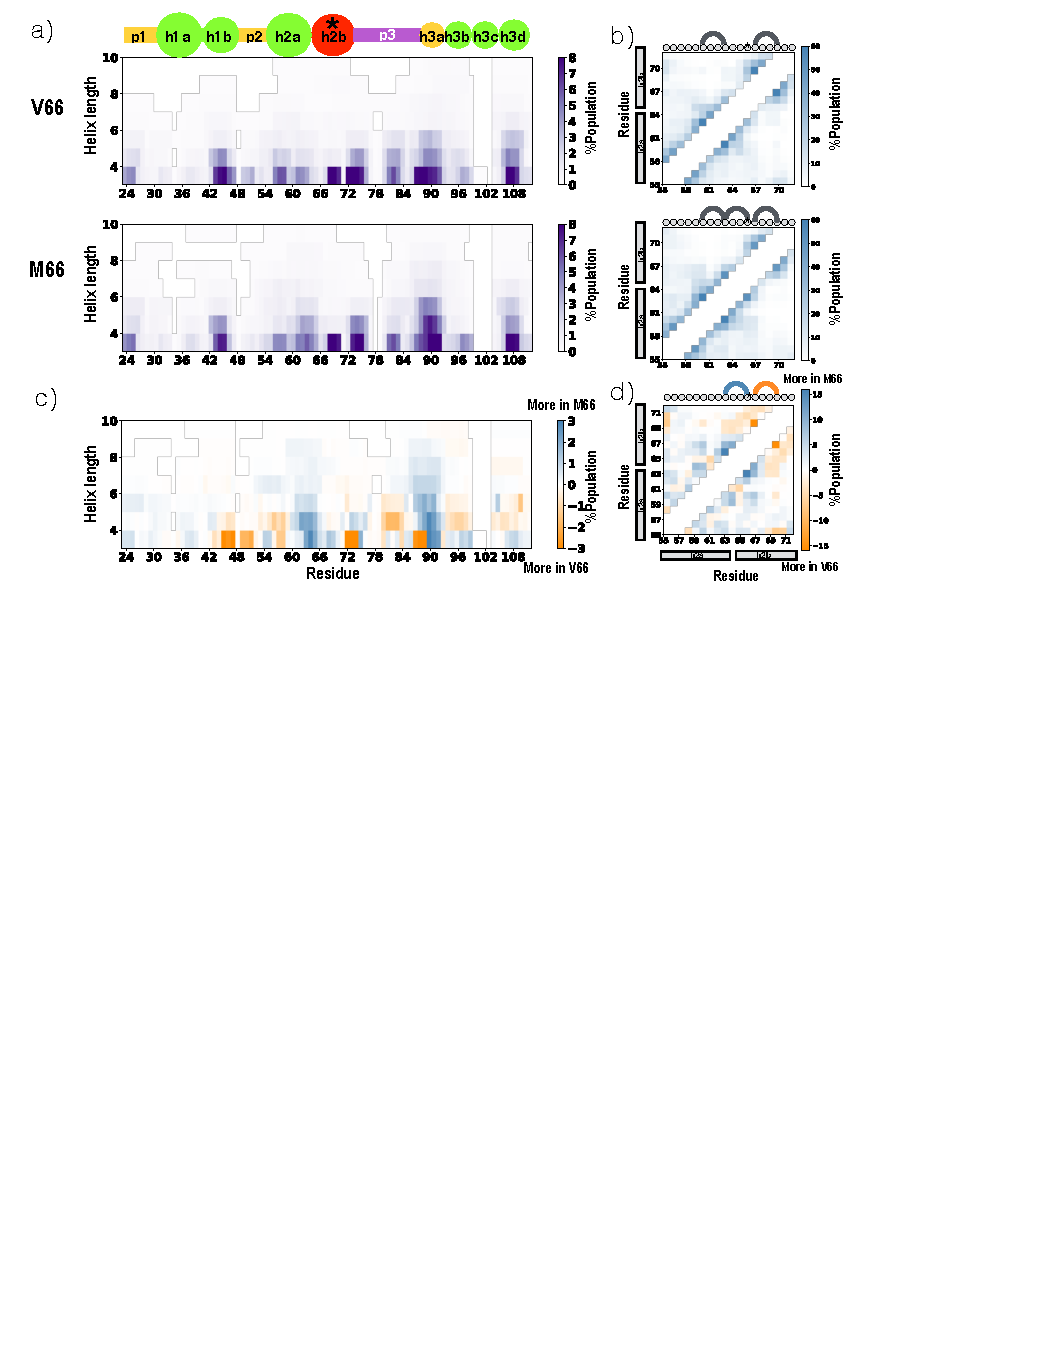
\includegraphics[scale=0.5,width=0.8\textwidth,trim={0 0cm 0 0cm},clip]{../figures/fig5.pdf}

\caption{{\bf Effects of Val66Met on intra-domain contacts at residue level.} a) Helix length probability at each residue and b) Contact probability for each residue pair within the h2 domain for V66 sequence (top) and M66 sequence (bottom). Each residue in domain h2 is annotated with a circle representation and the contacts with at-least 50\% population are represented with an edge. c) Difference in helix length probability shown in a), d) Difference between the contact probabilities shown in b); interactions more frequently found in M66 or V66 are in blue and orange respectively. }

\label{fig5} 
\end{figure}

In general, C\textsuperscript{$\beta$}-branched amino acids, such as Valine, have more restricted side-chain rotamers in helical conformation when compared with non-C\textsuperscript{$\beta$}-branched amino acids. Creamer et. al. ranked the entropic cost of helix formation for apolar side chains using simulations of a (Ala)\textsubscript{8} sequence with the guest amino acid at the center, and reported higher entropic cost of helix formation for Valine when compared with Methionine\cite{Creamer1992}. In our simulations, the likelihood that V66 will be in a short helix decreases with temperature, while the opposite effect is observed for M66 (Figure S6).
 
The helical structure in M66 is also stabilized by local sequence: the preferred interaction of Met66(i)-Phe63(i-3). MD simulations have previously shown the stability of a sulfur-aromatic contact in a model helix\cite{Viguera1995}. Figure~\ref{fig5}b shows the residue level contact map within domain h2. For the M66 sequence, Met66(i) is frequently contacting Phe63 (i-3) when compared with any other intra-domain contact at residue 66: M66-F63 is formed 60\% more often than M66-E69 (Figure~\ref{fig5}b). We find that the largest change in intra-domain contacts from V66 to M66 is the gain of contact at M66-F63 (40\% stronger in M66 when compared with V66) followed by loss of contact at Ile67 (i+1)-Leu70(i+4) (30\% weaker in M66 when compared with V66) (Figure~\ref{fig5}d). This is also consistent with previously identified Met-Phe interactions\cite{Viguera1995,Faure2008,Valley2012,Gomez-Tamayo2016}
%This is consistent with the results of ab-initio calculations: Gomez-Tamayo et al \cite{Gomez-Tamayo2016} identified Met-Phe interactions is stronger than Phe-Phe interactions. Bioinformatics screen of Protein DataBank (PDB) has repeatedly identified favorable Met-Phe contacts \cite{Viguera1995,Faure2008,Valley2012}
%Faure et al ~\cite {Faure2008} analyzed the frequency of two amino-acids contact within 1230 protein chains from the Protein DataBank (PDB) and found that Met residues are particularly likely to be contacting Phe and other Methionines.

 
%Among others 
%\subsubsection{Janus domain}
%QUESTIONS:
%In what way does the residual secondary structure or length of secondary structure elements change for each mutation and protonation state? (i.e. what should the reader be noticing)
%It was placed in the Janus sequence region based on f+ and f-, so are the changes in secondary structure associated with differences in interactions between charged residues? 
%END QUESTIONS

\subsection{Secondary structure coupling via tertiary interactions} 

%%%%Questions
% 1) In V66, there is a much stronger contact between h2b  and h3a  than in any of the other systems.  Are there ways in which the h2b  or h3a  intradomain interactions are also different for V66 from any of the other systems? [Provide 1-3 ways] 
% 2) For each difference, does the difference/correlation extend to fluctuations within the V66 sequence? (for example, one way might be that h3a  is also much less likely to form helix in V66 than the other sequences. Considering just the V66 simulation, for frames when 2b-3a contact is formed, are h3a  helices shorter/less probable than frames when no 2b-3a contact is formed?) 

%%%ON HOLD for now%---------residue level
%--Do the specific residues participating in interactions change for V66M, *particularly* *between within h2b  and 3a*
%--(optional) Do the specific residues participating in interactions change for 65+, *particularly* *between within h2b  and 3a* (edited).

While the effects of the Val66Met mutation on secondary structure in the domain (h2b) which contains residue 66 are not unexpected, we also observed a correlated effect on secondary structure in domain h3. As shown in Figure~\ref{fig2}c, the increased frequency of long helices for domain h3a in the Met66 sequence is comparable to the increase in domain h2b. This is consistent with NMR results ~\cite{Anastasia2013} showing a change in chemical shifts at residue 93 (Figure~\ref{fig2}c), although this effect was not originally discussed in Reference~\cite{Anastasia2013}. We hypothesized that since the Val66Met mutation affects the contact frequency between domain h2b and h3ab, the secondary structure change in h3ab could be due entirely to the change in these inter-domain contacts. To test this, we divided all frames into 4 clusters, representing two independent collective variables with two possible values each: either the h2b-h3a inter-domain contact is formed or broken, and either domain h2 does or does not contain a stretch of secondary structure of a given length. This clustering process on all frames was carried out twice, for each of two possible secondary structure elements (4 continuous residues in helix or 4 continuous residues in $\beta$). Populations of the individual clusters are shown in Table~\ref{table3}. The percent population of clusters with both respective secondary structure and h2b-h3a contact formed does not differ significantly from the uncorrelated expectation, also shown in Table~\ref{table3}.

\begin{table}[!ht]
\caption{Probabilities of simultaneous h2b-h3a interdomain contact and secondary structure formation in h2.  Each clustering process divided the frames based on two categorical variables with two possible values each: either the h2b-h3a inter-domain contact is formed or broken, and either domain h2 does or does not contain four contiguous residues in the given secondary structure.  Each sequence was clustered twice : once for helical secondary structure and once for $\beta$-strand. The expected cell frequencies, assuming no correlation, are shown in parenthesis. According to a Fisher exact test, $p > 0.01$ for all four contingency tables, even with generous estimates for the number of uncorrelated samples. 
 % incorporated  Errors represent standard error of a Bernoulli trial with n number of samples, where n is the product of total number of unique replicas in a given cluster and average number of roundtrips per replica, 17.
}
\label{table3}
%\begin{tabular}{|c|c|c|c|c|}
%\hline
%Contact h2b-h3a  &    \multicolumn{2}{c|}{V66 sequence} & \multicolumn{2}{c|}{M66 sequence}  \\ 
%\hline
%  &     helix   &  not helix   &  helix   &  not helix  \\
%\hline
%formed & 3.6 $\pm{0.8}$ (4.4) & 34.3 $\pm{1.5}$ (34.2) & 6.6 $\pm{1.0}$  (5.6) & 32.9 $\pm{1.5}$ (33.1)  \\
%\hline
%broken & 8.1 $\pm{0.9}$ (7.3) & 54.0 $\pm{1.5}$ (54.1) & 7.6 $\pm{1.0}$ (8.6) & 52.8 $\pm{1.5}$ (52.7) \\
%\hline
%\hline
% &   $\beta$     & not $\beta$   & $\beta$    & not $\beta$   \\
%\hline
%formed &   7.2  $\pm{ 0.9}$ (8.5) &   30.7 $\pm{1.5 }$ (30.4) &   10.7 $\pm{1.1}$ (9.2) &   28.9 $\pm{1.5}$ (29.2)  \\
%\hline
%broken&   15.2 $\pm{1.1}$ (13.9) &   46.9 $\pm{1.5}$ (47.2)  &   12.7 $\pm{1.1}$ (14.2) &   47.7 $\pm{1.4}$ (47.4) \\
%\hline
%
%\end{tabular}
\begin{tabular}{|c|c|c|c|c|}
 \hline
 &    \multicolumn{2}{c|}{V66 } & \multicolumn{2}{c|}{M66 }  \\ 
\hline
 &    \multicolumn{2}{c|}{h2 secondary structure}  & \multicolumn{2}{c|}{h2 secondary structure}   \\ 
\hline
  h2b-h3a contact &     helix   &  not helix   &  helix   &  not helix  \\
\hline
formed & 3.6 (4.4) & 34.3 (34.2) & 6.6 (5.6) & 32.9  (33.1)  \\
\hline
broken & 8.1 (7.3) & 54.0  (54.8) & 7.6  (8.6) & 52.8  (52.7) \\
\hline
\hline
 &   $\beta$     & not $\beta$   & $\beta$    & not $\beta$   \\
\hline
formed &   7.2  (8.5) &   30.7 (30.4) &   10.7 (9.2) &   28.9  (29.2)  \\
\hline
broken&   15.2 (13.9) &   46.9 (47.2)  &   12.7 (14.2) &   47.7 (47.4) \\
\hline
\end{tabular}
\end{table}

\begin{figure}[!ht]
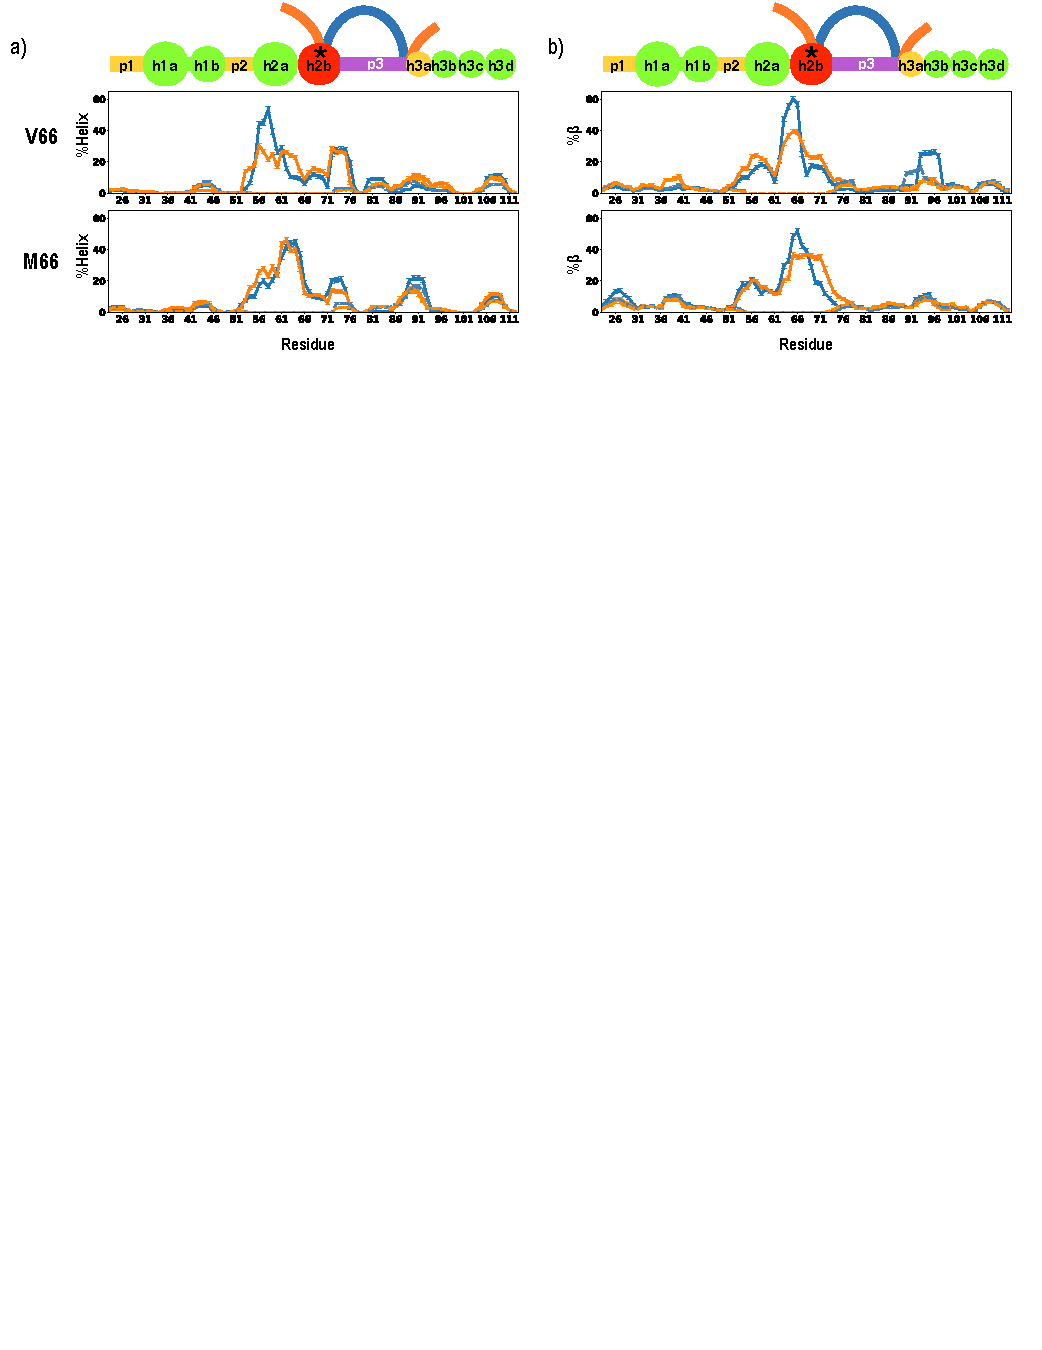
\includegraphics[scale=0.5,width=\textwidth,trim={0 0cm 0 0cm},clip]{../figures/fig6.pdf}
\caption{{\bf Secondary structure coupling between domains on each side of the p3 linker.} Helix (a) and $\beta$ (b) propensities at each residue in V66 sequence (top) and M66 sequence (bottom) for four clusters. Frames were first clustered by whether the inter-domain h2b-h3a contact was formed (blue) or broken (orange), and then by whether the respective secondary structure was present in h2 (solid) or absent (dashed). Errors represent standard error of a Bernoulli trial with n number of samples, where n is the product of total number of unique replicas in a given cluster and average number of roundtrips per replica, 17.
 }
\label{fig6}
\end{figure}


For any cluster, the secondary structure in the SNP-domain h2 is constrained by the clustering process. Helical or $\beta$ strand secondary structure propensities for all other residues, averaged across the frames in the cluster, are shown in Figure~\ref{fig6}. It would be very surprising to observe correlations in secondary structure between non-contacting domains in converged data; most likely such an observation would indicate a single dominant replica. Reassuringly, we detect no significant correlation of secondary structure in domains h2 and h3a unless the two domains are actually in contact: the orange solid and orange dashed lines overlap in Figure~\ref{fig6}. If our hypothesis was supported, h3a secondary structure would vary between clusters with and without the h2b-h3a contact (blue vs. orange lines in Figure~\ref{fig6} would not overlap) but would not depend on secondary structure in h2 (blue solid vs blue dashed lines in Figure~\ref{fig6} would overlap). Overall, we find that whether this hypothesis is supported for either helix-helix or $\beta$-$\beta$ coupling depends on whether residue 66 is Valine or Methionine.  


Figure~\ref{fig6}a compares the helix propensities at each residue for each cluster in the V66 and M66 sequences. In the V66 sequence, the clusters forming the h2b-h3a contact are less likely to be helical within h3a, regardless of whether h2 is in helix, supporting our original  hypothesis that the presence of the h2 domain was sufficient to affect the secondary structure of the ``context-sensitive''  Janus domain h3a. In the M66 sequence, when a helix is formed in h2 and h2b is in contact with domain h3a, h3a is more likely to form a helix than if domain h2 is not helical (Figure~\ref{fig6}a).  Furthermore, if domain h2 is not helical, helical propensity in domain h3a is indistinguishable from clusters in which the two domains are not even in contact. Thus, the interdomain contact is not sufficient to increase helical propensity: helix formation in domain h2 is also necessary for this effect in domain h3a. Consequently, our hypothesis is not supported for the M66 sequence. Overall, these results suggest that contact with the highly negatively charged h2b domain containing a Valine at residue 66 (regardless of its structure) is sufficient to slightly disrupt helical formation in the Janus domain h3a. When Val66 is replaced with Met, the interaction between the two domains becomes cooperative, consistent with helix-helix coupling.  

Few studies have reported helix-helix stabilization in IDPs. \citeauthor{Feuerstein2012}~\cite {Feuerstein2012} reported partly stabilized helical structure by long-range tertiary contacts in a disordered fragment of the hepatitis C virus protein NS5A with PRE measurement from NMR. \citeauthor{AlexanderConicella2016}~\cite {AlexanderConicella2016} showed that TDP-43 undergoes liquid-liquid phase separation in part via helical contacts that are enhanced by self-interaction and can be disrupted by disease mutation. However, identifying the type of interaction at residue level has been difficult due to disorder.

Interdomain coupling between $\beta$-strands is expected, even for disordered proteins: non-hairpin $\beta$-strand pairs cannot be local contacts. Any mutation in an IDP that disrupts local $\beta$-strand propensity should simultaneously reduce propensity of the partner strands. In the V66 sequence, we find that the h2b-h3a contact is associated with $\beta$-strand within h3a (Figure~\ref{fig6}b). In the M66 sequence, we do not observe any such correlation.
\begin{figure}[!ht]
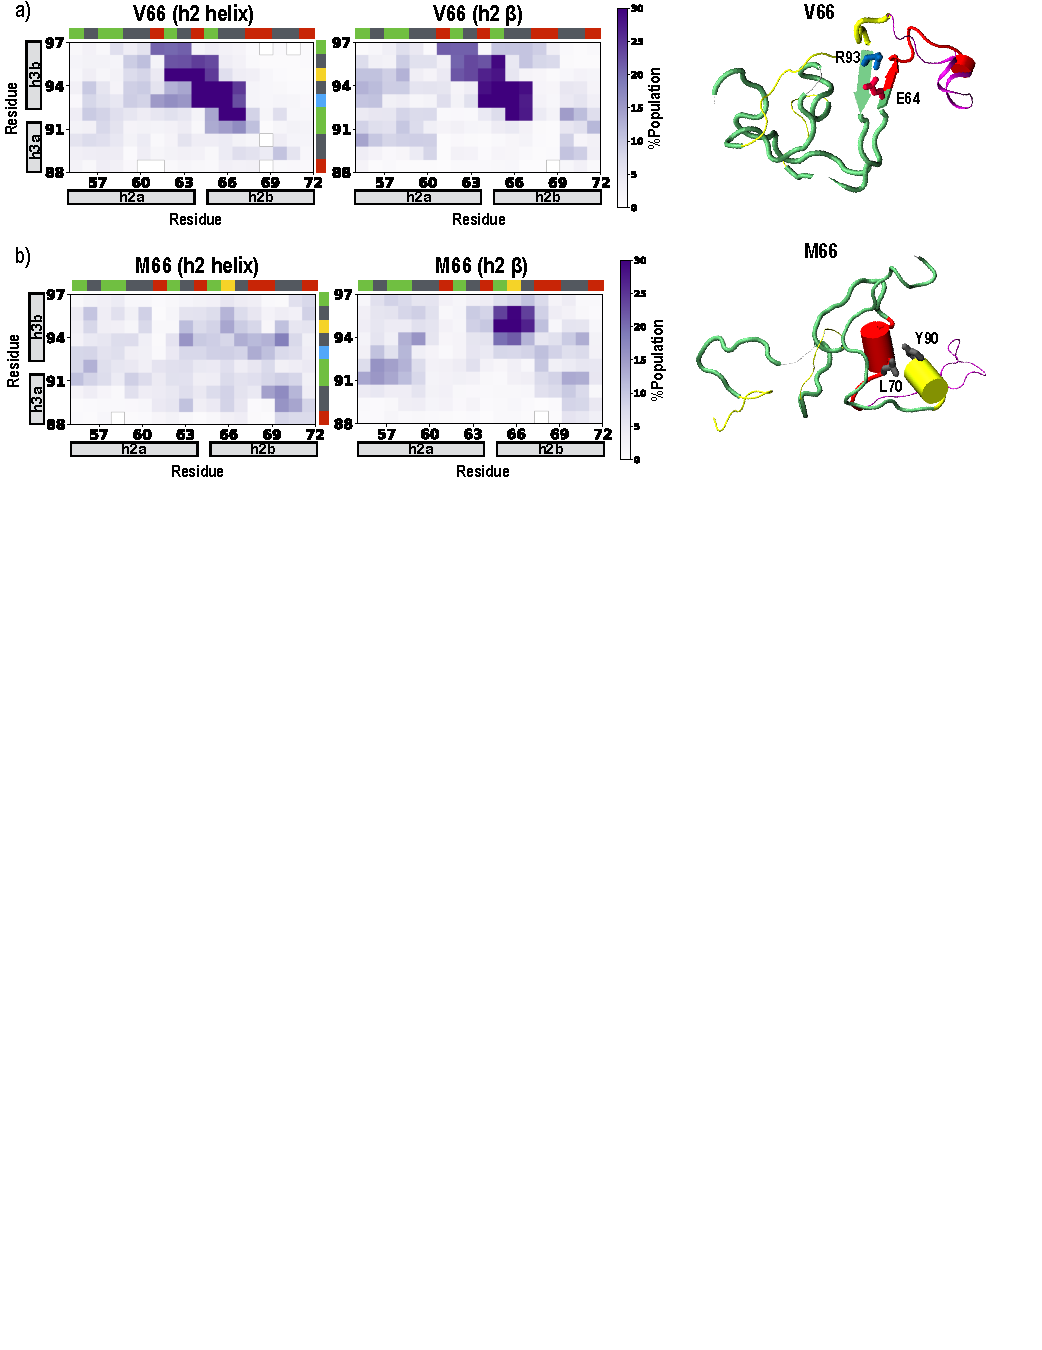
\includegraphics[scale=0.5,width=\textwidth,trim={0 0cm 0 0cm},clip]{../figures/fig7.pdf}
\caption{{\bf Effect of secondary structure in domain h2 on which residues form the cross-boundary h2-h3 contact.} Contact probability between each residue in h2 and h3ab, when h2 contains either helix (left) or $\beta$ (right) simultaneously with h2b-h3a contact, corresponding to the cluster represented by solid blue line in Figure~\ref{fig6}, for both the V66 (a) and M66 (b) sequences. Axes are annotated with boxes colored according to residue type: blue:basic, red:acidic, green:polar or Gly, grey:hydrophobic and Met: yellow. Representative conformations in V66 sequence (top) and M66 sequence (bottom) for each contact probability with chain colored as in Figure 1 and preferred residue-level contacts in Licorice representations, with residues colored by residue type.}
\label{fig7}
\end{figure}

%To summarize, we find that the direct contact between the SNP domain and h3ab predicts $\beta$ and helicity locally in V66 and M66 sequence respectively. This was further confirmed by looking at the intra-domain contact probability within h2 when either contact is formed for V66 vs M66 sequence (Figure~\ref{fig6}a). M66 sequence forms helix supporting contacts at residue 66(i) whereas V66 doesn't form any strong intra-domain contact at 66 when h2b-h3ab is formed.
%For non-local secondary structure change at h3ab, the h2b-h3ab inter-domain contact is necessary and but is not sufficient. Intra-domain contact at h2 influences intra-domain contact at h3ab when h2b-h3ab inter-domain contact is formed.

To determine which residue contacts between h2b and h3ab couple secondary structure within the two domains, we calculated the contact probability at residue level for the cluster with h2b-h3a contact and $\beta$ or helix within h2 for both sequences (Figure~\ref{fig7}). In the V66 sequence, 25\% of the frames  simultaneously forming the h2b-h3a contact and helix within h2 also form $\beta$ within h2. The $\beta$ pairing at h2b-h3ab is stabilized via combination of backbone hydrogen bonds between V66 and S92, salt bridge between E64 and R93, and hydrophobic interactions between V66 and V94 (Figure~\ref{fig7}a). In the M66 sequence, contact between h2 helices and h3ab is relatively unspecific and distributed among a number of possible hydrophobic contacts, particularly L70-Y90, as well as the M66-M95 interaction discussed in the previous section (Figure~\ref{fig7}b).

\section*{Summary and Conclusion}

We have carried out over 250 $\mu$s of fully-atomistic explicit solvent MD simulation of the 91 residue prodomain of brain-derived neurotrophic factor, with and without the disease-associated Val66Met mutation. These long simulations successfully reproduced the experimentally observed chemical shifts and $R_h$. The simulations also correctly reproduced the location of both local and non-local secondary changes due to the Val66Met mutation in the prodomain sequence. 

We find that the highly disordered 91 residue prodomain, which as a whole falls in the Janus sequence region of the \citeauthor{Das2013a} phase diagram~\cite{Das2013a}, can be meaningfully divided into 11 domains based on sequence hydrophobicity alone. Among 8 hydrophobic domains, we identified 2 domains in the disordered region: the strong polyelectrolyte domain h2b (which contains Val66Met), and the Janus domain h3a. These are connected via a highly disordered long linker region p3. These unique domains have biological significance as well: The sequence h2-p3-h3 is essential for intracellular trafficking of proBDN~\cite {Chen2005}. 

The domain decomposition suggested a tractable approach for coarse-graining analysis, by reducing the initial number of potential contacts from over 4000 to 55, while increasing the number of observations for each contact. Furthermore, it allowed us to isolate the most useful regions of the protein for examination at the residue level. This domain decomposition method, simply based on sequence hydrophobicity, may be a generally useful strategy to identify functionally significant regions in proteomics investigations for any long disordered proteins, and our conclusions suggest an important role for disorder heterogeneity within disordered proteins. 

We were able to identify mechanisms through which a charge-neutral mutation can affect a disordered proteins residual secondary structure and tertiary contacts, as well as how these effects can be propagated to non-local residual secondary structure.  Within domain h2b the Val66Met mutation affects intra-domain contact preference due to local sequence effects (preferred Met-Phe contacts) and the reduced entropic cost of helix formation for the Methionine sidechain. Consistent with the sequence characteristics of Janus sequences, we find that the secondary structure of the Janus domain h3a is sensitive to contacts with the highly charged h2b domain. For the Met66 sequence, this sensitivity is only observed when the contacting h2b domain is also helical.  We did not detect such extreme sensitivity in other domains, although the entire prodomain does fall in the Janus region on the \citeauthor{Das2013a} diagram in Figure \ref{fig1}b. Thus, this designation may only be predictive for shorter segments of the sequence that would also fall in the Janus region on their own.  
%h2b-h3a contacts favor helix-helix coupling between the two domains in M66 whereas in V66 this contact breaks helicity at h3a. 

The long, disordered, exposed p3 linker segregates the inter-domain contact probability map: domains on the same side of p3 have a high probability of contact whereas probability of contact between either side of p3 is less probable.  We consistently observed this segregation in both simple self-avoiding hetropolymer simulations with beads mimicking identified domains, and actual prodomain simulations. Val66Met increases the frequency of contacts between domains on either side of p3 due to favorable Met-Met or Met-Phe contacts. These interactions have been shown to stabilize tertiary contacts in folded proteins and membrane proteins, but their role has not been investigated in disordered proteins. In general, our study supports the observation that Methionine is distinct from generic hydrophobic residues due to the presence of polarizable Sulphur~\cite{Gomez-Tamayo2016, Lim2019}. 

\citeauthor{Anastasia2013}~\cite{Anastasia2013} observed differential kinetics for interactions between the BDNF prodomain and SorCS2; M66 binds more preferably at the SNP domain h2b (H65 to L71) with SorCS2, whereas V66 binds weakly overall but more strongly with domain h3a and h3b (residues Y90 to V94). The stronger binding at residue M66 could be attributed to either A) Helix propensity at the SNP domain in M66. This SNP domain helix segregates all the acidic and hydrophobic residues on either side of helix. Therefore, it is likely that this preformed structure will be helpful for binding B) preferred Met-Met contacts when compared with Val-Met contacts. We find frequent interactions of Met66 with the only other Methionine in the prodomain, and the SorCS2 surface is rich in exposed methionines\cite{Leloup2018}. Therefore, it is possible that the M66 prodomain binds strongly to SorCS2 due to preferred Met-Met contacts between residue Met66 and the SorCS2 Met residues or a combination of both A) and B). This hypothesis could be tested experimentally by mutation of the methionines in SorCS2.  

\section*{Materials and Methods}

\subsection*{System setup} To account for differences in starting coil conformation, we included six unique structures to represent residues 23-113 of BDNF prodomain.  All structures were built using I-Tasser~\cite{Yang2014,Roy2010,Bioinformatics}, Rosetta~\cite{Kim2004} and Modeller~\cite{Sali1993a}, and all were simulated in a water box at 600K for 50 ns at a constant volume. From the six resulting trajectories, 64 structures with correct proline isomers were selected (based on at least 2ps time interval); in total, our study included 64 unique prodomain structures. All structures were cooled to 300K for 1ns, while prolines were restrained in trans-conformation. Each V66 replica was placed in a dodecahedron water box with 30,500 TIP4P-D ~\cite{Piana2015} water molecules and a 0.15M salt concentration (NaCl) for a total system size of approximately 124,000 atoms. The same volume for each replica was ensured by fixing the simulation box of each replica to the average box size (11 nm).

\subsection*{Molecular Dynamics Simulation} For the simulations we use the amber99SB*-ILDN-q force field\cite{Lindorff-Larsen2010a, Hornak2006a} and the GROMACS 5.1.2 simulation package,\cite{Berendsen1995,Abraham2015} with a time step of 2 fs. Long-range electrostatics are calculated using the particle mesh Ewald (PME) method~\cite{Essmann1995}, with a 1 nm cutoff and a 0.12 nm grid spacing. Periodic boundary conditions are also used to reduce system size effects. System was simulated using T-REMD\cite{Sugita1999a} with an exchange frequency of 1ps for 2 $\mu$s, giving a total simulation time of 128~$\mu$s with NVT ensemble for each system. 64 replicas are used with temperatures ranging from 300-385K, with exponential spacing. A different random seed was used for the Langevin dynamics of each replica. The average exchange acceptance probability ranged between 0.19-0.23. 

The minimum separation between the molecule and its image was less than 2 nm only \textless 1\% of the time for both sequences and these frames were discarded from all the analysis. Time-series of the relative measurements were generated every 100 ps. For both V66 and M66 groups, initial 0.5 $\mu$s (800 ns $\times$ 64) were discarded for equilibration purposes, determined by plateauing of $R_h$ (Figure~\ref{fig2}b). Over the course of remaining 76.8 $\mu$s (1.2 $\mu$s $\times$ 64) simulations, for both the V66 and M66 sequence each replica completes a minimum of 5 roundtrips and an average of 17 roundtrips (Figure S7). 
 
Time-series of the radius of gyration $R_g$ and end-to-end distance $R_{\mathrm{etoe}}$ were calculated using respectively the g\textunderscore gyrate and g\textunderscore polystat utilities of Gromacs. We took $R_{\mathrm{etoe}}$ as the distance between N-termini and C-termini N and O atoms respectively. Statistical uncertainties are provided for $R_g$, $R_h$ as total standard deviation divided by the square root of the product of total number of replicas (64) and average number of roundtrips per replica, 17.  

%M - .36, V- .77, V-hip-11, 4.47 , replica 38 becomes expanded, all the frames from this replica is removed giving 1.66 remaining replicas, M-hip-11, 1.16. 
\subsection*{Domain identification} Mean hydrophobicity ($\langle H\rangle$) at each residue is defined as the average Kyte-Dolittle\cite{Kyte1982a} score with a window size of 3 residues, scaled to fit between 0 and 1. Any stretch of four or more residues with $\langle H \rangle$ of 0.37 or more is classified as hydrophobic domain and from the remaining residues, stretch of four or more residues is classified as linker region.

\subsection*{Chemical Shifts calculation}  Prior to the present study, ~\citeauthor{Anastasia2013}\cite{Anastasia2013} measured chemical shifts for the BDNF prodomain (residues 21-113) using NMR, and then used backbone NMR chemical shifts to predict secondary structure via TALOS+ ~\cite{Shen2009} and SSP~\cite{Marsh2006a}. For comparison with simulation data, we reinterpreted the chemical shifts directly from\cite{Anastasia2013}, deposited at Biological Magnetic Resonance Bank. Random coil reference chemical shifts were obtained from the Poulsen IDP/IUP random coil chemical shifts\cite{Schwarzinger2001,Kjaergaard2011b,Kjaergaard2011a} at pH 7, 280 K.

\subsection*{Hydrodynamic radius calculation} 
The values for the Hydropro ~\cite {Ortega2011} parameters were: atomic level model with shell-method calculation, a = 0.29 nm, 6 minibead iterations, $\sigma$ = 0.1 to 0.2 nm. The temperature was taken to be 300 K, the solvent viscosity 0.01 Poise, the solvent density 1.0 $gcm^\mathrm{-3}$, the partial specific volume of the peptide 0.7313 $cm^\mathrm{3}g^\mathrm{-1}$ (V66 sequence) or 0.7304 $cm^\mathrm{3}g^\mathrm{-1}$ (M66 sequence), and a molecular weight of the peptide equal to 10044 Da (V66 sequence) or 10076 Da (M66 sequence).

\subsection*{Secondary structure calculation} Helix propensity or $\beta$ propensity is expressed as the probability of a given residue being part of a sequence of four consecutive residues whose dihedral angles place them in the helical region or $\beta$ region of the Ramachandran space. The helical region is defined as -100$^{\circ}$  \textless $\phi$ \textless -30$^{\circ}$  and -120$^{\circ}$ \textless $\psi$ \textless 50$^{\circ}$ \cite{Nodet,Garcia2002,Knott2012b}. The $\beta$ region is defined as $\phi$ \textless -80$^{\circ}$  and 50$^{\circ}$  \textless $\psi$ \textless -120$^{\circ}$. The length of SS (SS-map) \cite{Iglesias2013} were calculated with the above defined helical and $\beta$ region. The error bars are calculated with standard error of a Bernoulli trial with n number of samples, where n is the product of total number of unique replicas in a cluster and average number of roundtrips per replica, 17.


\subsection*{Self-avoiding heteropolymer simulation} 
The BDNF prodomain was approximated as a freely-jointed self-excluding heteropolymer with 11 monomers, each mimicking one of the domains identified in Figure~\ref{fig1}.  The separation between monomers $i$ and $i+1$ (analogous to the Kuhn length for a homopolymer~\cite{Rubinstein2003}) was constrained to be half the end to end distance for each of the analogous domains:

\begin{equation}|\vec{r}_{i-1} - \vec{r}_i| = \frac{\langle R_{etoe,i-1}\rangle +  \langle R_{etoe,i}\rangle }{2}\label{eq:bond}\end{equation}

where $\langle R_{etoe,i}\rangle$ was determined from the coordinates of domain $i$ residues in the MD simulations, given in Table~\ref{table2}.

Two monomers $i$ and $j$ are considered to be overlapping if \begin{equation}|\vec{r}_i- \vec{r}_j| < a (\langle R_{g, i}\rangle + \langle R_{g, j}\rangle)\label{eq:overlap}\end{equation} where $\langle R_{g, i}\rangle$ was determined from the coordinates of residues in domain $i$ in the MD simulations (Table~\ref{table2}), and $a$ is a constant.  In the MD simulations of the real protein, we observed that the center of mass distances between domains were rarely less than $0.3~(\langle R_{g, i}\rangle + \langle R_{g, j}\rangle)$, and thus we set $a =0.3$.

The random walk was carried out using a simple Metropolis Monte Carlo, with the following move set: 1) a random bead $i>0$ was selected,  2)  a random displacement vector $\vec{\delta r}$ was generated in three cartesian dimensions, 3) $\vec{\delta r}$ was scaled so that $|\vec{r}_{i-1} - (\vec{r}_i + \vec{\delta r})| =( \langle R_{etoe,i-1}\rangle + \langle R_{etoe,i}\rangle)/2$, satisfying Eq \ref{eq:bond}, 4) the translation $\vec{r}_j \rightarrow \vec{r_j} + \delta_r$ was applied for all $j\ge i$.

Any trial move that caused an overlap according to Eq. \ref{eq:overlap} was rejected, while all others were accepted.  The MC simulation was run for 50,000 steps (50,000 for each moveable bead); additional steps did not change the outcome in Figure~\ref{fig3}.

\subsection*{Contact maps}
Two domains $i$ and $j$ are in contact if the excess distance ($d_{\mathrm{e,ij}}$) between the two is less than 0.55 nm, where excess distance is defined as $d_{\mathrm{e,ij}} =  \sqrt{(\vec{r}_i - \vec{r}_j)^2} - (R_{\mathrm{g,i}}+R_{\mathrm{g,j}})$, $\vec{r}_i$ is the position vector of a domain $i$ defined as the mean of its N-termini N atom and C-termini O atom coordinates, calculated using g\textunderscore traj utility of Gromacs. Two residues are in contact if the distance between C\textsubscript{$\alpha$}-C\textsubscript{$\alpha$} atoms between the two residues is 0.8 nm or less. Statistical uncertainties are calculated as total standard deviation of a given contact formation divided by the square root of the product of total number of replicas forming the given contact and average number of roundtrips per replica, 17.


\section*{Acknowledgments}
The authors are grateful to Dr. Clay Bracken and Dr. Barbara Hempstead of Weill Cornell Medical Center for helpful discussions. Computational time was provided through XSEDE resources via NSF MCB110149 and the Rutgers Discovery Informatics Institute, which are supported by Rutgers and the State of New Jersey~\cite{Parashar2018}.

%\begin{suppinfo}
\section*{Supporting Information Available}
Figures showing comparison of various force field and NMR chemical shifts; comparison of M66 sequence chemical shifts with NMR chemical shifts; Ensemble averaged interchain distance profiles for V66 sequence for each domain; Effect of perturbing monomer properties on freely-jointed, self-avoiding heteropolymer; Residue level contacts for the entire prodomain; Effects of temperature and Val66Met mutation on helix propensity around residue 66; Number of round trip completed by each replica; a table of fitted Flory exponents for each domain.

%\end{suppinfo}


%%%%%%%%%%%%%%%%%%%%%%%%%%%%%%%%%%%%%%%%%%%%%%%%%%%%%%%%%%%%%%%%%%%%%
%% The appropriate \bibliography command should be placed here.
%% Notice that the class file automatically sets \bibliographystyle
%% and also names the section correctly.
%%%%%%%%%%%%%%%%%%%%%%%%%%%%%%%%%%%%%%%%%%%%%%%%%%%%%%%%%%%%%%%%%%%%%
\bibliography{Jacs_ref}


%%%%%%%%%%%%%%%%%%%%%%%%%%%%%%%%%%%%%%%%%%%%%%%%%%%%%%%%%%%%%%%%%%%%%
%% The appropriate \bibliography command should be placed here.
%% Notice that the class file automatically sets \bibliographystyle
%% and also names the section correctly.
%%%%%%%%%%%%%%%%%%%%%%%%%%%%%%%%%%%%%%%%%%%%%%%%%%%%%%%%%%%%%%%%%%%%%
%\bibliography{achemso-demo}




\end{document}